% !TEX program = xelatex
% ============================================================
%  全国大学生数学建模竞赛 (CUMCM) LaTeX 论文
%  编译方式: XeLaTeX
% ============================================================
\documentclass[12pt,a4paper]{ctexart}

% ======================== 宏包加载 ========================
\usepackage[top=2.5cm, bottom=2.5cm, left=2.5cm, right=2.5cm]{geometry}
\usepackage{amsmath, amssymb, amsthm}
\usepackage{graphicx}
\usepackage{float}
\usepackage{subcaption}
\usepackage{booktabs}
\usepackage{array}
\usepackage{multirow}
\usepackage{longtable}
\usepackage{xcolor}
\usepackage{hyperref}
\hypersetup{
    colorlinks=true,
    linkcolor=blue!70!black,
    citecolor=green!50!black,
    urlcolor=blue!60!black
}
\usepackage{listings}
\lstset{
    basicstyle=\small\ttfamily,
    breaklines=true,
    frame=single,
    numbers=left,
    numberstyle=\tiny\color{gray},
    keywordstyle=\color{blue},
    commentstyle=\color{green!60!black},
    stringstyle=\color{red!70!black},
    tabsize=4
}

\usepackage{setspace}
\onehalfspacing
\usepackage{enumitem}
\setlist{nosep, leftmargin=2em}
\usepackage[indentafter]{titlesec}
\usepackage{caption}
\captionsetup{font=bf}
\usepackage{bm}
\usepackage{mathtools}

% ======================== 字体设置 ========================
\setCJKmainfont{SimSun}[BoldFont=SimHei, ItalicFont=KaiTi]
\setCJKsansfont{SimHei}
\setCJKmonofont{FangSong}
\setmainfont{Times New Roman}
\setCJKfamilyfont{zhsong}{SimSun}[BoldFont=SimHei]
\setCJKfamilyfont{zhhei}{SimHei}[BoldFont=SimHei]
\setCJKfamilyfont{zhkai}{KaiTi}[BoldFont=SimHei]
\setCJKfamilyfont{zhfang}{FangSong}[BoldFont=SimHei]

% ======================== 编号格式 ========================
\renewcommand{\thesection}{\chinese{section}、}
\renewcommand{\thesubsection}{\arabic{section}.\arabic{subsection}}
\renewcommand{\thesubsubsection}{\arabic{section}.\arabic{subsection}.\arabic{subsubsection}}

% ======================== 标题格式 ========================
\titleformat{\section}
  {\centering\heiti\zihao{-3}\bfseries}
  {\thesection}{0em}{}
\titlespacing*{\section}{0pt}{1.5ex plus .5ex minus .2ex}{1.0ex plus .2ex}

\titleformat{\subsection}
  {\heiti\zihao{4}\bfseries}
  {\thesubsection}{1em}{}
\titlespacing*{\subsection}{0pt}{1.2ex plus .4ex minus .2ex}{0.8ex plus .2ex}

\titleformat{\subsubsection}
  {\heiti\zihao{-4}\bfseries}
  {\thesubsubsection}{1em}{}
\titlespacing*{\subsubsection}{0pt}{1.0ex plus .3ex minus .1ex}{0.6ex plus .1ex}

% ======================== 定理环境 ========================
\theoremstyle{definition}
\newtheorem{definition}{定义}[section]
\newtheorem{assumption}{假设}[section]
\theoremstyle{plain}
\newtheorem{theorem}{定理}[section]
\newtheorem{lemma}{引理}[section]
\newtheorem{proposition}{命题}[section]
\newtheorem{corollary}{推论}[section]
\theoremstyle{remark}
\newtheorem{remark}{注}[section]

% ======================== 自定义命令 ========================
\renewenvironment{abstract}
  {\begin{center}\heiti\zihao{-3}摘\quad 要\end{center}\zihao{-4}\songti\indent}
  {\par\vspace{1em}}

\newcommand{\keywords}[1]{%
  \par\noindent\textbf{关键词：}#1}

\newenvironment{symboltable}
  {\begin{center}\zihao{5}\begin{tabular}{>{\centering\arraybackslash}p{3.5cm} p{7.5cm} >{\centering\arraybackslash}p{1.5cm}}
  \toprule
  \textbf{符号} & \textbf{含义} & \textbf{单位} \\
  \midrule}
  {\bottomrule\end{tabular}\end{center}}

\newcommand{\step}[1]{\par\noindent\textbf{Step #1}\quad}

% ============================================================
\begin{document}
\pagestyle{plain}

\begin{center}
{\zihao{-2}\heiti\bfseries 微网与外部电网电力调控策略}
\end{center}
\vspace{1em}

% ======================== 摘要 ========================
\setcounter{page}{1}
\pagenumbering{arabic}

\begin{abstract}
本文针对微网与外部电网的电力调控策略优化问题，综合运用混合整数线性规划（MILP）、滚动优化与多阶段调整策略等方法，建立了系统化的购电决策模型。

\textbf{针对问题一：}在电价与负载固定、光伏发电预测已知的条件下，建立了以全天购电费用最小化为目标的MILP模型。模型以144个10分钟时段为决策周期，引入充放电互斥二进制变量精确刻画储能设备物理特性，采用HiGHS求解器精确求解。最终得到全天最优购电费用为$35\,126.95$元，购电量$59\,482.70$~kWh，相较于无储能方案节省$26.90\%$。

% 后续问题的摘要待补充
\end{abstract}

\keywords{微网调度；混合整数线性规划；储能优化；分时电价；滚动优化}

% ============================================================
%  正文
% ============================================================

\section{问题重述}

\subsection{问题背景}
微网是为促进光伏发电等分布式能源的就地消纳、缓解并网冲击而迅速发展的小型发用电系统。出于经济考量，非孤岛式微网可在外部电网（下文简称外网）电价偏低或分布式能源有多余电量的时段，为储能设备充电蓄能，并在外网电价较高的时段放电。

微网与外网的调控目的是综合利用小区负载、光伏发电功率及储能设备的当前储电量等信息，尽可能精准地决策微网的购电量与储能设备的充放电量，使得微网所供电力既能满足小区的负载需求，又尽可能节约购电费用。
\subsection{问题提出}

已知微网的电价数据、小区负载数据、光伏发电功率数据以及储能设备的物理参数，其中储能设备的最大容量为$12\,000$~kWh，最大充放电功率为$5\,000$~kW，初始储电量为$6\,000$~kWh，储电量约束为$[1\,200, 10\,800]$~kWh，充放电效率为$90\%$。本文需要解决以下问题：

\textbf{问题一：}若每天的电价和小区负载相同，且光伏发电功率预测已知，要求微网提供的电能不低于小区负载，且储能设备在$0{:}00$和$24{:}00$的储电量相同，在每天$0{:}00$制定当天的计划购电策略。

\textbf{问题二：}若每天电价相同，而小区负载和光伏发电功率随时间变化，且当实际供电低于负载时需以$5$倍电价紧急购电，在每天$0{:}00$制定当天的计划购电策略。

\textbf{问题三：}在每天$0{:}00$、$6{:}00$、$12{:}00$和$18{:}00$可获得未来24小时光伏发电功率预报，可据此调整购电策略。调整涉及违约费用和超购费用，减少部分按$50\%$电价收费，增加部分按$1.5$倍电价收费，建立微网当天购电策略的数学模型。

\textbf{问题四：}在电价也实时波动的情况下，重新计算问题二和问题三的购电策略。


\section{问题分析}

\subsection{问题一的分析}

问题一要求在给定电价、负载和光伏预测数据的条件下，制定微网当天的最优计划购电策略，以最小化全天总购电费用。由于储能充放电会直接改变各时段的外购电需求，两变量相互耦合，因此模型需将各时段的外购电量与储能充放电量作为联合决策变量，在保证各时段供电不低于小区负载、储能充放电功率与剩余电量均不超出设备允许范围、且首尾电量一致的物理约束下，寻找全局最优的电量分配方案。考虑到储能设备不可同时充放电的特性需引入 0-1 状态变量刻画，以及目标函数与主要约束均为线性关系，本问构建混合整数线性规划（MILP）模型；由于单日时段规模有限，采用 HiGHS 求解器可快速求得全局最优解，从而输出各时段的最优购电量与储能调度策略。

\begin{figure}[H]
  \centering
  \begin{subfigure}[b]{0.48\textwidth}
    \centering
    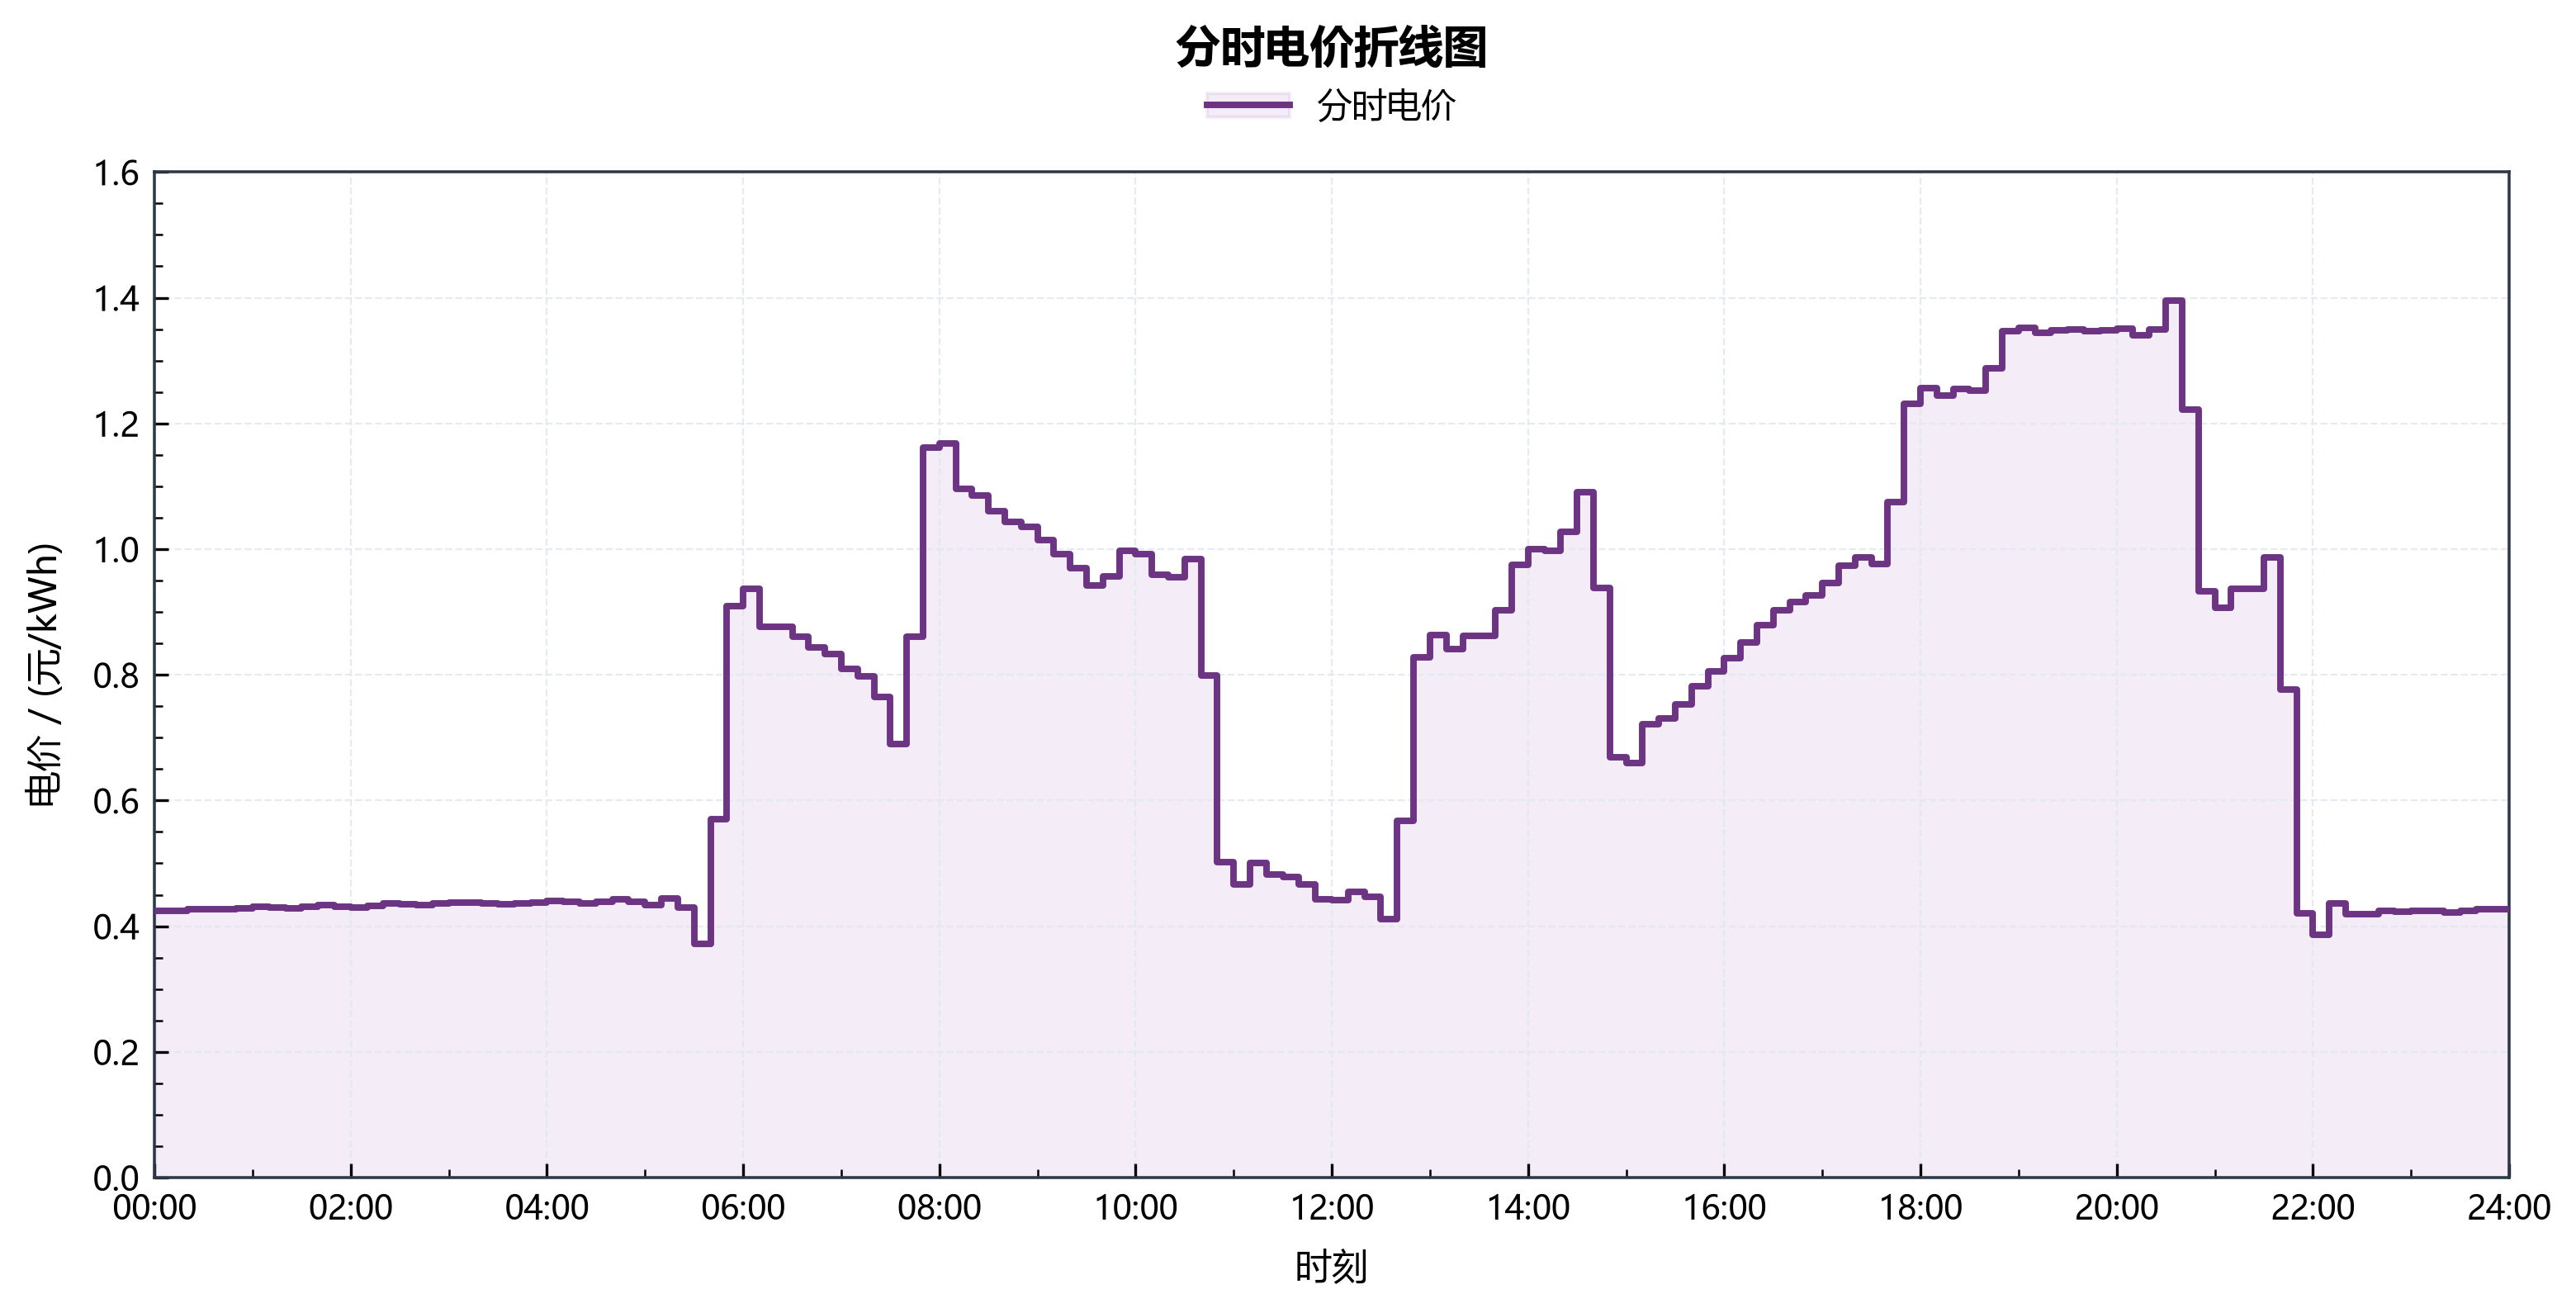
\includegraphics[width=\textwidth]{../../C题/问题一可能用到的图片/分时电价折线图.png}
    \caption{附件1分时电价曲线}
    \label{fig:q1_input_price}
  \end{subfigure}
  \hfill
  \begin{subfigure}[b]{0.48\textwidth}
    \centering
    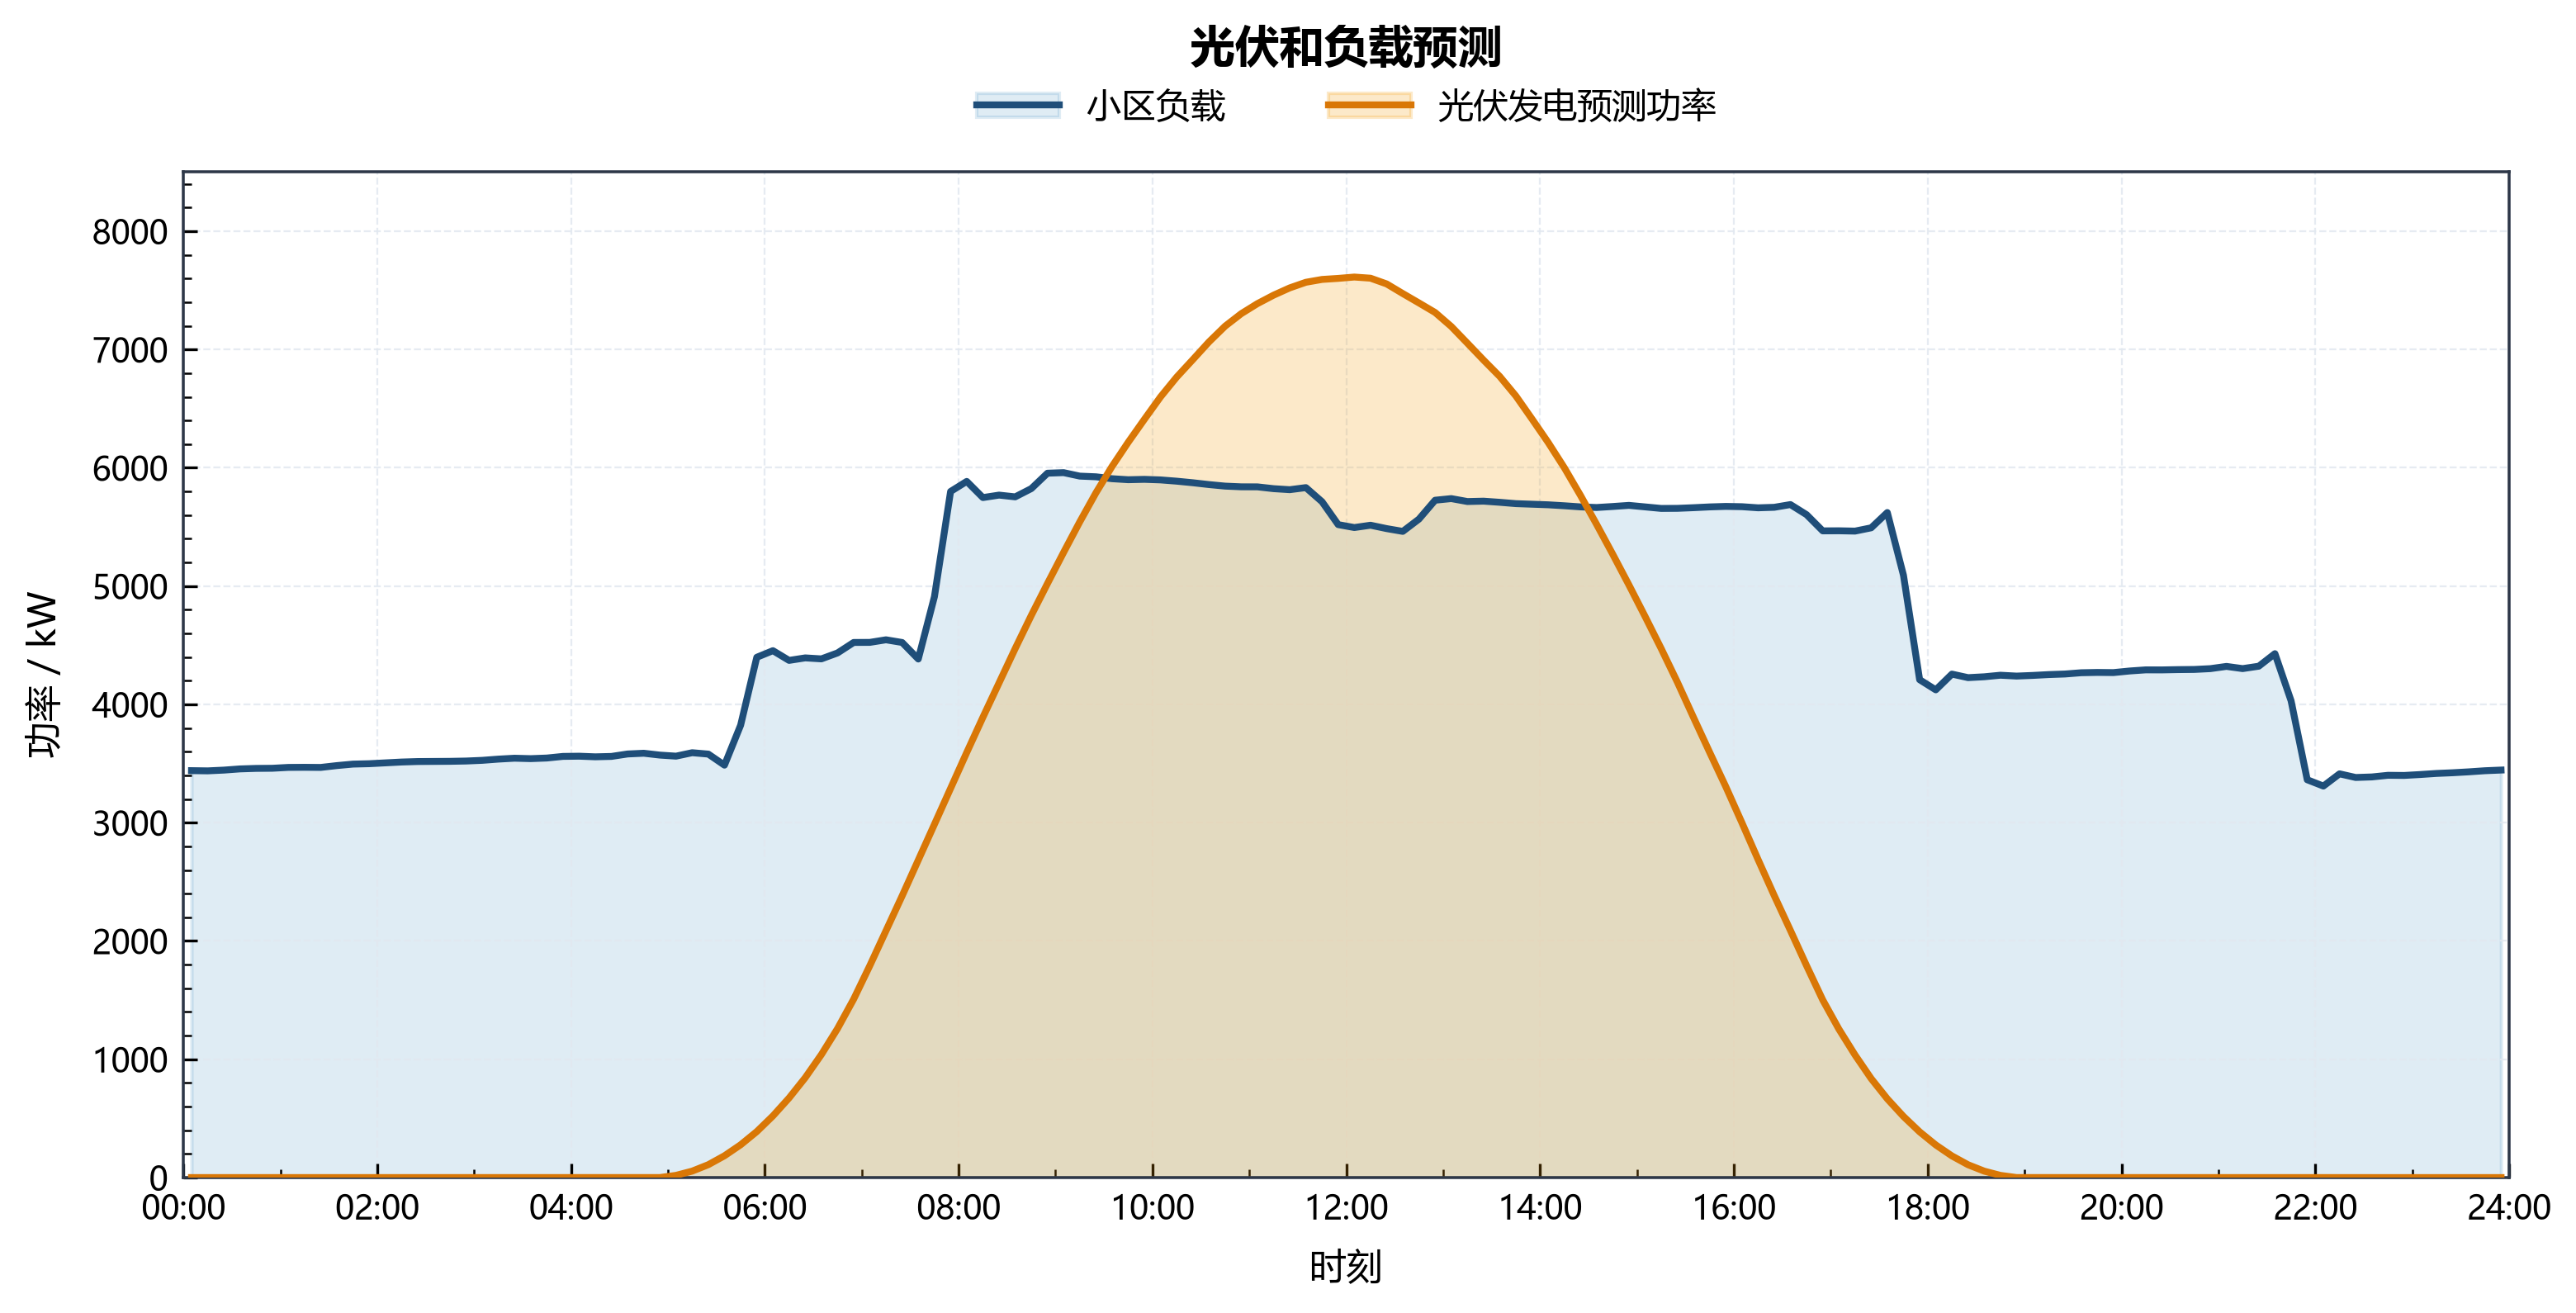
\includegraphics[width=\textwidth]{../../C题/问题一可能用到的图片/光伏和负载预测.png}
    \caption{附件1负载与光伏预测曲线}
    \label{fig:q1_input_load_pv}
  \end{subfigure}
  \caption{附件1的电价、负载与光伏预测数据}
  \label{fig:q1_input_data}
\end{figure}

\subsection{问题二的分析}
问题二要求在每天0:00、当日真实负载与光伏尚未知的条件下决定当天144个时段的购电计划，使334天内的计划购电费与应急购电费之和最小。由于计划不足需高价购电来应急，且溢出部分虽不退款但可贮存留用，低估代价远高于高估；本问在继承问题一规划模型的基础上新增预测环节，估计当日光伏与负载功率。我们将其拆解为预测、日前计划与真实数据反馈三个模块：在预测模块中，我们先依据小区负载的周内规律与光伏发电日间规律做季节性朴素预测；再根据历史数据构造时序特征，采用LightGBM回归模型对季节性预测结果做进一步修正；最后以该各时段历史残差的的高分位数再次修正，以此来减少不可避免的低估造成的影响。随后以修正净需求与当日实际初态为输入，将计划购电量、名义充放电量及充放电状态作为决策变量，建立以计划费最小为目标的日前混合整数线性规划模型；做出计划后，逐段揭示真实供需情况，对富余电量进行贮存、并在用电缺口时进行放电、不足时购买应急电量并跨日继承状态，从而在保证小区用电需求的情况下尽可能降低用电成本。因模型与问题一同为线性且含互斥0-1变量，仍采用HiGHS求解器求解，并回测输出全年购电计划、应急安排与总费用。
\subsection{问题三的分析}
问题三在问题二日前计划的基础上引入每日四次的未来 24 小时光伏预报，购电决策由当天的单次日前计划扩展为多时刻滚动修订；增购部分按电价 1.5 倍计费，减购部分按电价 50\% 计违约费，因此需要判断更新预报带来的收益能否补偿两类调整费用，并以全天普通购电、计划调整和应急购电的总费用最小为目标。为解决该问题，本问沿用问题二预测、计划修订与执行反馈的框架：预测部分继续采用问题二的负载预测，并将附件 3 整点预报转换为 10 分钟区间，结合历史预测误差进行修正；计划修订部分仅对剩余未交付时段重新求解混合整数线性规划，并满足供电平衡、储能递推、充放电互斥及储电量边界约束，每次更新只用当前已发布预报和真实储电量，仅当修订后的预计总费用更低时才采用新计划；执行部分仍按实际供需逐段反馈并跨日继承储电量。最后设置三组对照，通过比较三组总费用与应急购电量，分别评估更换预报来源与引入日内购电修订的收益。
\subsection{问题四的分析}
% 待补充


\section{模型假设}

\begin{enumerate}[label=\arabic*.]
\item 微网向外部电网的购电即时且足额，任意时段缺口均可按当时电价立即购入，无传输延迟与购电上限.
\item 微网不具备售电能力，外购电量非负，多余电力只能弃置或存入储能。
\item 储能无自放电损耗，未充放电的时段储电量保持不变；充放电效率恒为90\%且不随充放电功率和荷电状态变化。
\item 每个10分钟时段内负载功率与光伏发电功率保持恒定，以该时段采样值作为区间代表值并乘时段长度折算为电量。
\item 每日0:00的决策仅使用此前已结束区间的观测与已发布预测，当日实际负载与光伏逐段揭示.
\item 2025年1月作为冷启动预运行期以积累残差样本与电池初态，不计入评价。
\end{enumerate}


\section{符号说明}

\begin{symboltable}
$t$ & 时段编号，$t = 0, 1, \ldots, 143$ & -- \\
$\Delta t$ & 时段长度，$\Delta t = 1/6$ 小时 & h \\
$p_t$ & 第$t$个时段的电价 & 元/kWh \\
$L_t$ & 第$t$个时段的小区负载功率 & kW \\
$V_t$ & 第$t$个时段的光伏发电功率 & kW \\
$L_t^{E}$ & 第$t$个时段的负载电量，$L_t^{E} = L_t \cdot \Delta t$ & kWh \\
$V_t^{E}$ & 第$t$个时段的光伏电量，$V_t^{E} = V_t \cdot \Delta t$ & kWh \\
$q_t$ & 第$t$个时段的计划购电量 & kWh \\
$c_t$ & 第$t$个时段储能设备母线侧充电量 & kWh \\
$d_t$ & 第$t$个时段储能设备母线侧放电量 & kWh \\
$w_t$ & 第$t$个时段的弃电量 & kWh \\
$z_t$ & 充放电状态指示变量，$z_t \in \{0, 1\}$ & -- \\
$E_t$ & 第$t$个时段起始时刻的储能设备内部储电量 & kWh \\
$\eta_c$ & 储能设备充电效率，$\eta_c = 0.9$ & -- \\
$\eta_d$ & 储能设备放电效率，$\eta_d = 0.9$ & -- \\
$P_{\max}$ & 储能设备最大充放电功率，$P_{\max} = 5000$ & kW \\
$M$ & 单时段最大充放电电量，$M = P_{\max} \cdot \Delta t$ & kWh \\
\end{symboltable}


\section{模型建立与求解}

\subsection{问题一模型建立及求解}

\begin{figure}[H]
  \centering
  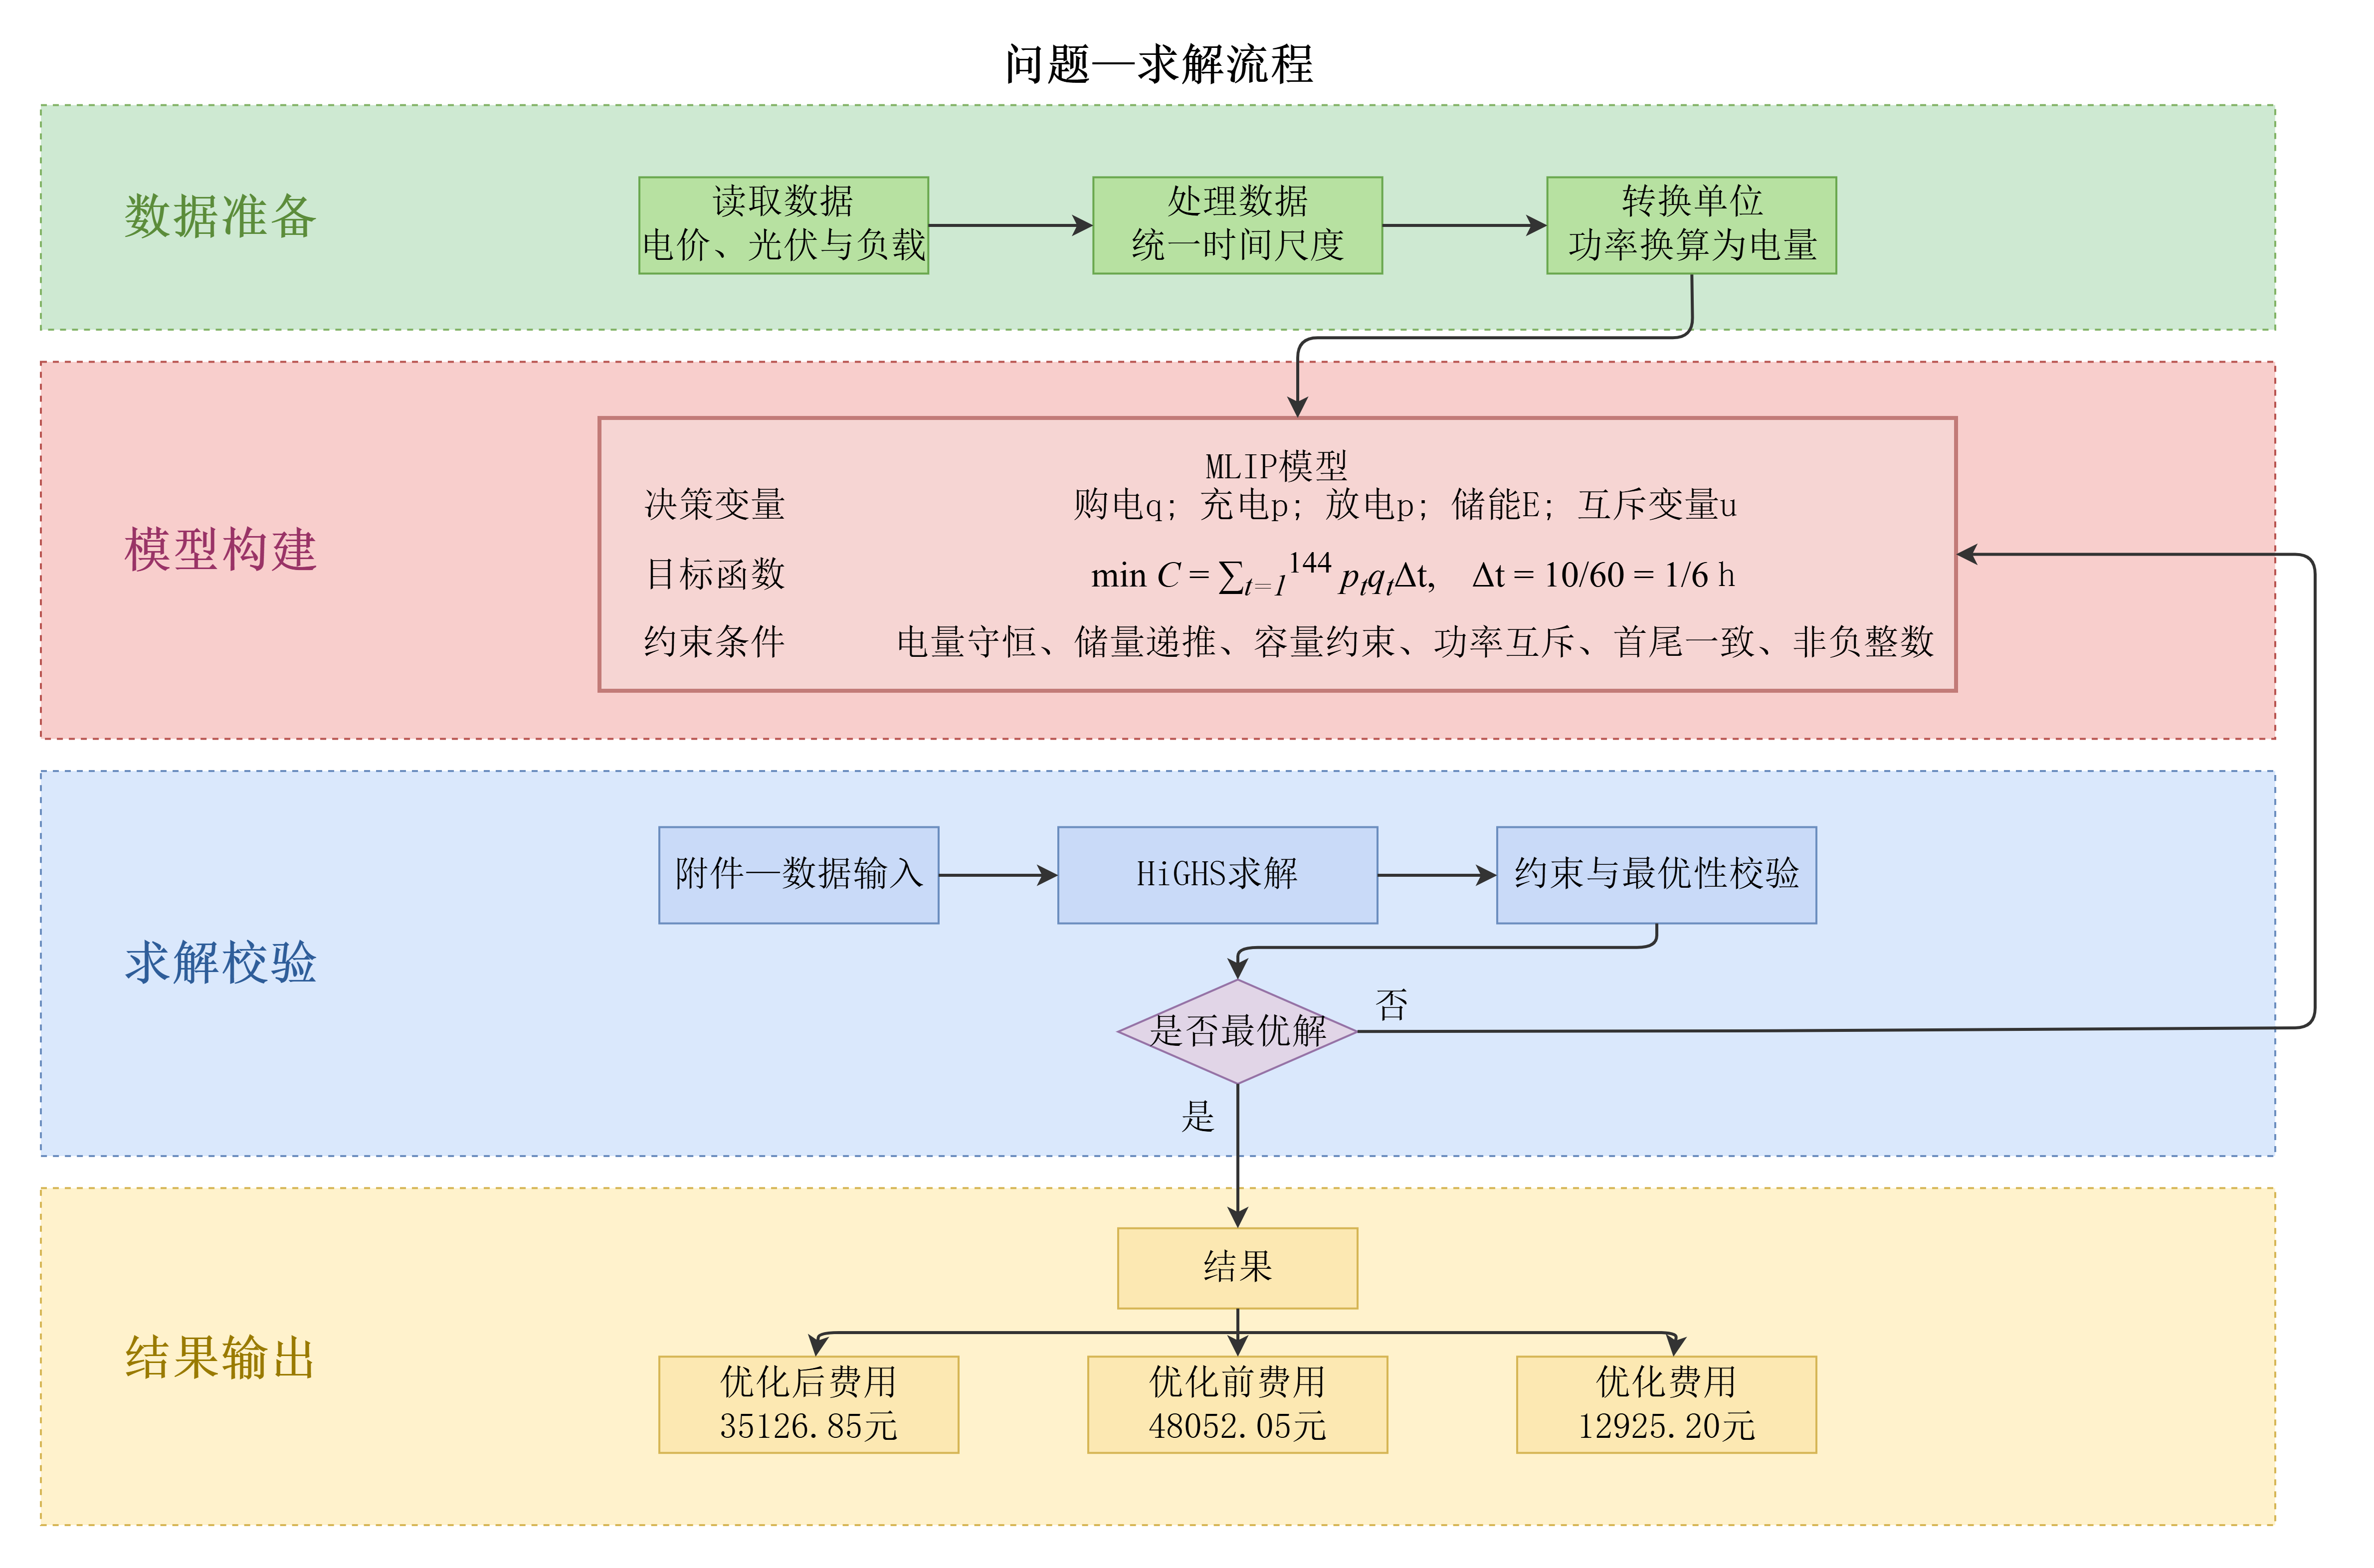
\includegraphics[width=0.9\textwidth]{../../C题/问题一可能用到的图片/修改版流程图.png}
  \caption{问题一模型求解流程}
  \label{fig:q1_solution_flow}
\end{figure}

\subsubsection{数据预处理}

附件 1 提供了一天内 144 个等间隔时刻的电价、小区负载功率及光伏发电预测功率数据。本文将每个采样值作为其前 10 分钟区间的代表值，采样值 0:10 代表 0:00–0:10 这一时段，24:00 代表 23:50–24:00。时段内的电价与功率取该标签处的采样值并视为恒定。记时段编号为$t=0,1,\ldots,143$，第$t$个时段对应从第$10t$分钟到第$10(t+1)$分钟的区间。

由于数据以功率（kW）形式给出，而优化模型需要以电量（kWh）为决策变量，因此需进行如下转换。设时段长度$\Delta t = \frac{10}{60} = \frac{1}{6}$小时，则第$t$个时段的负载电量和光伏发电电量分别为：
\begin{equation}
  L_t^{E} = L_t \cdot \Delta t, \quad V_t^{E} = V_t \cdot \Delta t
  \label{eq:q1_energy_convert}
\end{equation}
\noindent 其中$L_t$和$V_t$分别为第$t$个时段的负载功率和光伏发电功率。

\subsubsection{模型建立}

\noindent\textbf{（1）决策变量}\\[6pt]
\indent 为完整描述微网在每个时段的电力调度过程，令调度时段$t = 0, 1, \ldots, 143$，定义连续决策变量$q_t, c_t, d_t, w_t \geq 0$和二元决策变量$z_t \in \{0, 1\}$。其中$z_t = 1$表示储能设备处于充电模式，$z_t = 0$表示放电模式，用于避免同一时段同时充放电。

此外，定义状态变量$E_t$为第$t$个时段开始前储能设备的内部储电量（kWh），$t = 0, 1, \ldots, 144$，其中$E_0$为初始储电量，$E_{144}$为调度周期结束时的储电量。

\noindent\textbf{（2）目标函数的确定}\\[6pt]
\indent 微网的全天购电费用等于各时段购电量与对应电价之积的总和。以最小化全天购电费用为目标：
\begin{equation}
  \min \quad Z = \sum_{t=0}^{143} p_t \cdot q_t
  \label{eq:q1_obj}
\end{equation}
\noindent 其中$p_t$为第$t$个时段的电价（元/kWh）。由于充放电的费用已经通过其对购电量的影响计入购电费用，储能变量只进入约束而不直接进入目标函数，避免重复计费。

\noindent\textbf{（3）约束条件}\\[6pt]
\noindent\textbf{a. 母线电量平衡约束}\\[4pt]
\indent 题目要求微网提供的电能不可低于小区负载。在各时段，购电量、光伏发电量与储能放电量之和，必须等于小区负载、储能充电量与未使用电量之和，保证微网能量平衡：
\begin{equation}
  q_t + V_t^{E} + d_t = L_t^{E} + c_t + w_t, \quad t = 0, 1, \ldots, 143
  \label{eq:q1_bus_balance}
\end{equation}
其中，$q_t$ 为计划购电量，$V_t^{E}$ 与 $L_t^{E}$ 分别为光伏和负载电量，$c_t, d_t$ 分别为母线侧充电量和放电量，$w_t$ 为未使用电量。

\noindent\textbf{b. 储能设备储电量递推约束}\\[4pt]
\indent 储能设备的充放电效率按单向各 $90\%$ 计算。充电时存入内部电量为 $0.9 c_t$，放电时内部消耗电量为 $d_t / 0.9$，由此确定相邻时段电池内部储电量的递推关系：
\begin{equation}
  E_{t+1} = E_t + \eta_c \cdot c_t - \frac{d_t}{\eta_d} = E_t + 0.9 \, c_t - \frac{d_t}{0.9}, \quad t = 0, 1, \ldots, 143
  \label{eq:q1_soc_dynamics}
\end{equation}
其中，$E_t$ 为时段起点储能设备内部的储电量。

\noindent\textbf{c. 储能设备容量范围约束}\\[4pt]
\indent 附录1规定，为了避免过度充电或放电，储能设备的储电量在全天所有时段必须始终保持在 1200--10800~kWh 之间：
\begin{equation}
  1200 \leq E_t \leq 10\,800, \quad t = 0, 1, \ldots, 144
  \label{eq:q1_soc_bounds}
\end{equation}

\noindent\textbf{d. 充放电功率与互斥约束}\\[4pt]
\indent 储能设备的最大充放电功率为 $5000\text{ kW}$，单时段充放电量上限为 $M = 5000 \times \frac{1}{6} = 833.\overline{3}\text{ kWh}$。显式引入二进制变量 $z_t \in \{0, 1\}$ 限制储能设备不可同时充放电，其中$z_t=1$表示允许充电、$z_t=0$表示允许放电：
\begin{equation}
  0 \leq c_t \leq M \cdot z_t, \quad 0 \leq d_t \leq M \cdot (1 - z_t), \quad t = 0, 1, \ldots, 143
  \label{eq:q1_charge_discharge_limit}
\end{equation}

\noindent\textbf{e. 日初日末储电量相同约束}\\[4pt]
\indent 题目要求储能设备在 $0:00$ 和 $24:00$ 的储电量相同，结合附录1给定的初始储电量 $6000\text{ kWh}$，首末储电量满足：
\begin{equation}
  E_0 = E_{144} = 6000\text{ kWh}
  \label{eq:q1_boundary}
\end{equation}

\noindent\textbf{f. 变量非负与整数约束}\\[4pt]
\indent 购电量与未使用电量必须非负，充放电状态变量取二进制整数：
\begin{equation}
  q_t \geq 0, \quad w_t \geq 0, \quad z_t \in \{0, 1\}, \quad t = 0, 1, \ldots, 143
  \label{eq:q1_nonneg}
\end{equation}

\noindent\textbf{（4）完整模型汇总}\\[6pt]
\indent 综合上述分析，问题一的MILP模型可完整表述为：

\begin{equation}
\begin{aligned}
  \min \quad & \boxed{Z = \sum_{t=0}^{143} p_t \cdot q_t} \\[6pt]
  \text{s.t.} \quad 
  & \left.
  \begin{aligned}
    & q_t + V_t^{E} + d_t = L_t^{E} + c_t + w_t \\
    & E_{t+1} = E_t + 0.9\,c_t - \frac{d_t}{0.9} \\
    & 0 \leq c_t \leq 833.\overline{3} \cdot z_t \\
    & 0 \leq d_t \leq 833.\overline{3} \cdot (1 - z_t) \\
    & q_t \geq 0, \quad w_t \geq 0, \quad z_t \in \{0, 1\}
  \end{aligned}
  \right\} \quad t = 0, 1, \ldots, 143 \\[6pt]
  & 1200 \leq E_t \leq 10\,800, \quad t = 0, 1, \ldots, 144 \\[4pt]
  & E_0 = E_{144} = 6000
\end{aligned}
\label{eq:q1_full_model}
\end{equation}


\subsubsection{模型求解}

本问采用优化求解器HiGHS~\cite{huangfu2018parallelizing}对上述MILP模型进行精确求解。由于目标函数与全部约束均为线性，充放电互斥只需引入0-1变量即可线性刻画，问题一属于标准的混合整数线性规划，采用分支定界法即可获得全局最优解；HiGHS集成了单纯形法、内点法和分支定界法，能够高效处理该规模共865个变量的MILP，对该尺寸问题可在秒级内精确求解并获得全局最优证认，无需依赖遗传算法等随机搜索方法。

依据式~\eqref{eq:q1_full_model}构建MILP模型，定义目标函数和全部约束条件，调用HiGHS求解器进行求解。目标函数下界与最优值完全一致，均为$35\,126.95$元。

模型的各项物理一致性校验结果如表~\ref{tab:q1_validation}所示，所有指标均在数值精度范围内满足约束要求。

\begin{table}[H]
\centering
\caption{问题一MILP模型求解结果的物理一致性校验}
\label{tab:q1_validation}
\zihao{5}
\begin{tabular}{lc}
\toprule
\textbf{校验指标} & \textbf{数值} \\
\midrule
母线能量平衡最大绝对误差（kWh）  & $1.71 \times 10^{-13}$ \\
储电量递推最大绝对误差（kWh）    & $8.74 \times 10^{-13}$ \\
储电量边界违反量（kWh）          & $0.00$ \\
充放电流量越界违反量（kWh）      & $0.00$ \\
充放电互斥违反量（kWh）          & $0.00$ \\
二进制变量完整性误差             & $9.10 \times 10^{-15}$ \\
\bottomrule
\end{tabular}
\end{table}

\subsubsection{结果展示}

\paragraph{（1）全天关键指标}

问题一模型的最优调度策略下，全天关键运行指标如表~\ref{tab:q1_summary}所示。

\begin{table}[H]
\centering
\caption{问题一最优调度策略的全天关键指标}
\label{tab:q1_summary}
\zihao{5}
\begin{tabular}{lc}
\toprule
\textbf{指标} & \textbf{数值} \\
\midrule
全天购电费（元）             & $35\,126.95$ \\
全天购电量（kWh）            & $59\,482.70$ \\
全天充电量（kWh）            & $20\,740.67$ \\
全天放电量（kWh）            & $16\,799.94$ \\
弃电量（kWh）                & $0.00$ \\
初始储电量 $E_0$（kWh）      & $6\,000.00$ \\
最终储电量 $E_{144}$（kWh）  & $6\,000.00$ \\
\bottomrule
\end{tabular}
\end{table}

全天负载总电量为$111\,024.8$~kWh，光伏发电总电量为$55\,482.8$~kWh，净负载电量为$55\,542.0$~kWh。最优方案的购电量$59\,482.70$~kWh高于净负载电量，其差值$3\,940.70$~kWh恰好对应储能设备充放电过程中$\eta_c \cdot \eta_d = 0.81$所带来的往返能量损耗，即$19\%$。

\paragraph{（2）指定时段购电量}

按题目要求，表~\ref{tab:q1_purchase_specified}给出指定时段的购电量以及全天购电量和购电费用。

\begin{table}[H]
\centering
\caption{微网在指定时间段的购电量及全天购电量和购电费}
\label{tab:q1_purchase_specified}
\zihao{5}
\begin{tabular}{cc|cc|cc}
\toprule
\textbf{时间段} & \textbf{购电量(kWh)} & \textbf{时间段} & \textbf{购电量(kWh)} & \textbf{时间段} & \textbf{购电量(kWh)} \\
\midrule
$10{:}00$--$10{:}10$ & $0.000$ & $12{:}00$--$12{:}10$ & $480.412$ & $14{:}00$--$14{:}10$ & $0.000$ \\
$16{:}00$--$16{:}10$ & $445.432$ & $18{:}00$--$18{:}10$ & $531.894$ & $20{:}00$--$20{:}10$ & $0.000$ \\
\midrule
\multicolumn{2}{c|}{\textbf{全天购电量(kWh)}} & \multicolumn{4}{c}{$59\,482.70$} \\
\multicolumn{2}{c|}{\textbf{全天购电费(元)}} & \multicolumn{4}{c}{$35\,126.95$} \\
\bottomrule
\end{tabular}
\end{table}

\paragraph{（3）储能设备充放电量及储电量}

表~\ref{tab:q1_storage}给出储能设备在各4小时时段的充放电量以及$0{:}00$和$24{:}00$的储电量。

\begin{table}[H]
\centering
\caption{储能设备在指定时间段的充放电量及$0{:}00$和$24{:}00$的储电量}
\label{tab:q1_storage}
\zihao{5}
\begin{tabular}{ccc|ccc}
\toprule
\textbf{时间段} & \textbf{充电量(kWh)} & \textbf{放电量(kWh)} & \textbf{时间段} & \textbf{充电量(kWh)} & \textbf{放电量(kWh)} \\
\midrule
$0{:}00$--$4{:}00$   & $4\,500.00$ & $0.00$      & $4{:}00$--$8{:}00$   & $833.33$    & $6\,365.84$ \\
$8{:}00$--$12{:}00$  & $4\,787.96$ & $1\,703.00$ & $12{:}00$--$16{:}00$ & $5\,286.04$ & $91.10$     \\
$16{:}00$--$20{:}00$ & $0.00$      & $5\,780.13$ & $20{:}00$--$24{:}00$ & $5\,333.33$ & $2\,859.87$ \\
\midrule
\multicolumn{3}{c|}{$0{:}00$储电量\;(kWh)：$6\,000.00$} & \multicolumn{3}{c}{$24{:}00$储电量\;(kWh)：$6\,000.00$} \\
\bottomrule
\end{tabular}
\end{table}

\paragraph{（4）全天购电策略与调度时序分析}

全天购电策略的核心特征可以从时序图中直接观察。图~\ref{fig:q1_dispatch_overview}给出全天购电功率、充电功率与放电功率的变化，图~\ref{fig:q1_operation_curve}给出负载、光伏、母线功率、储电量与电价的同步关系。购电功率在凌晨谷价时段维持高位，白天光伏盈余时段降为零，傍晚高价时段由储能放电替代购电，深夜再恢复购电补充储能，形成"谷充峰放"的调度时序。

\begin{figure}[H]
  \centering
  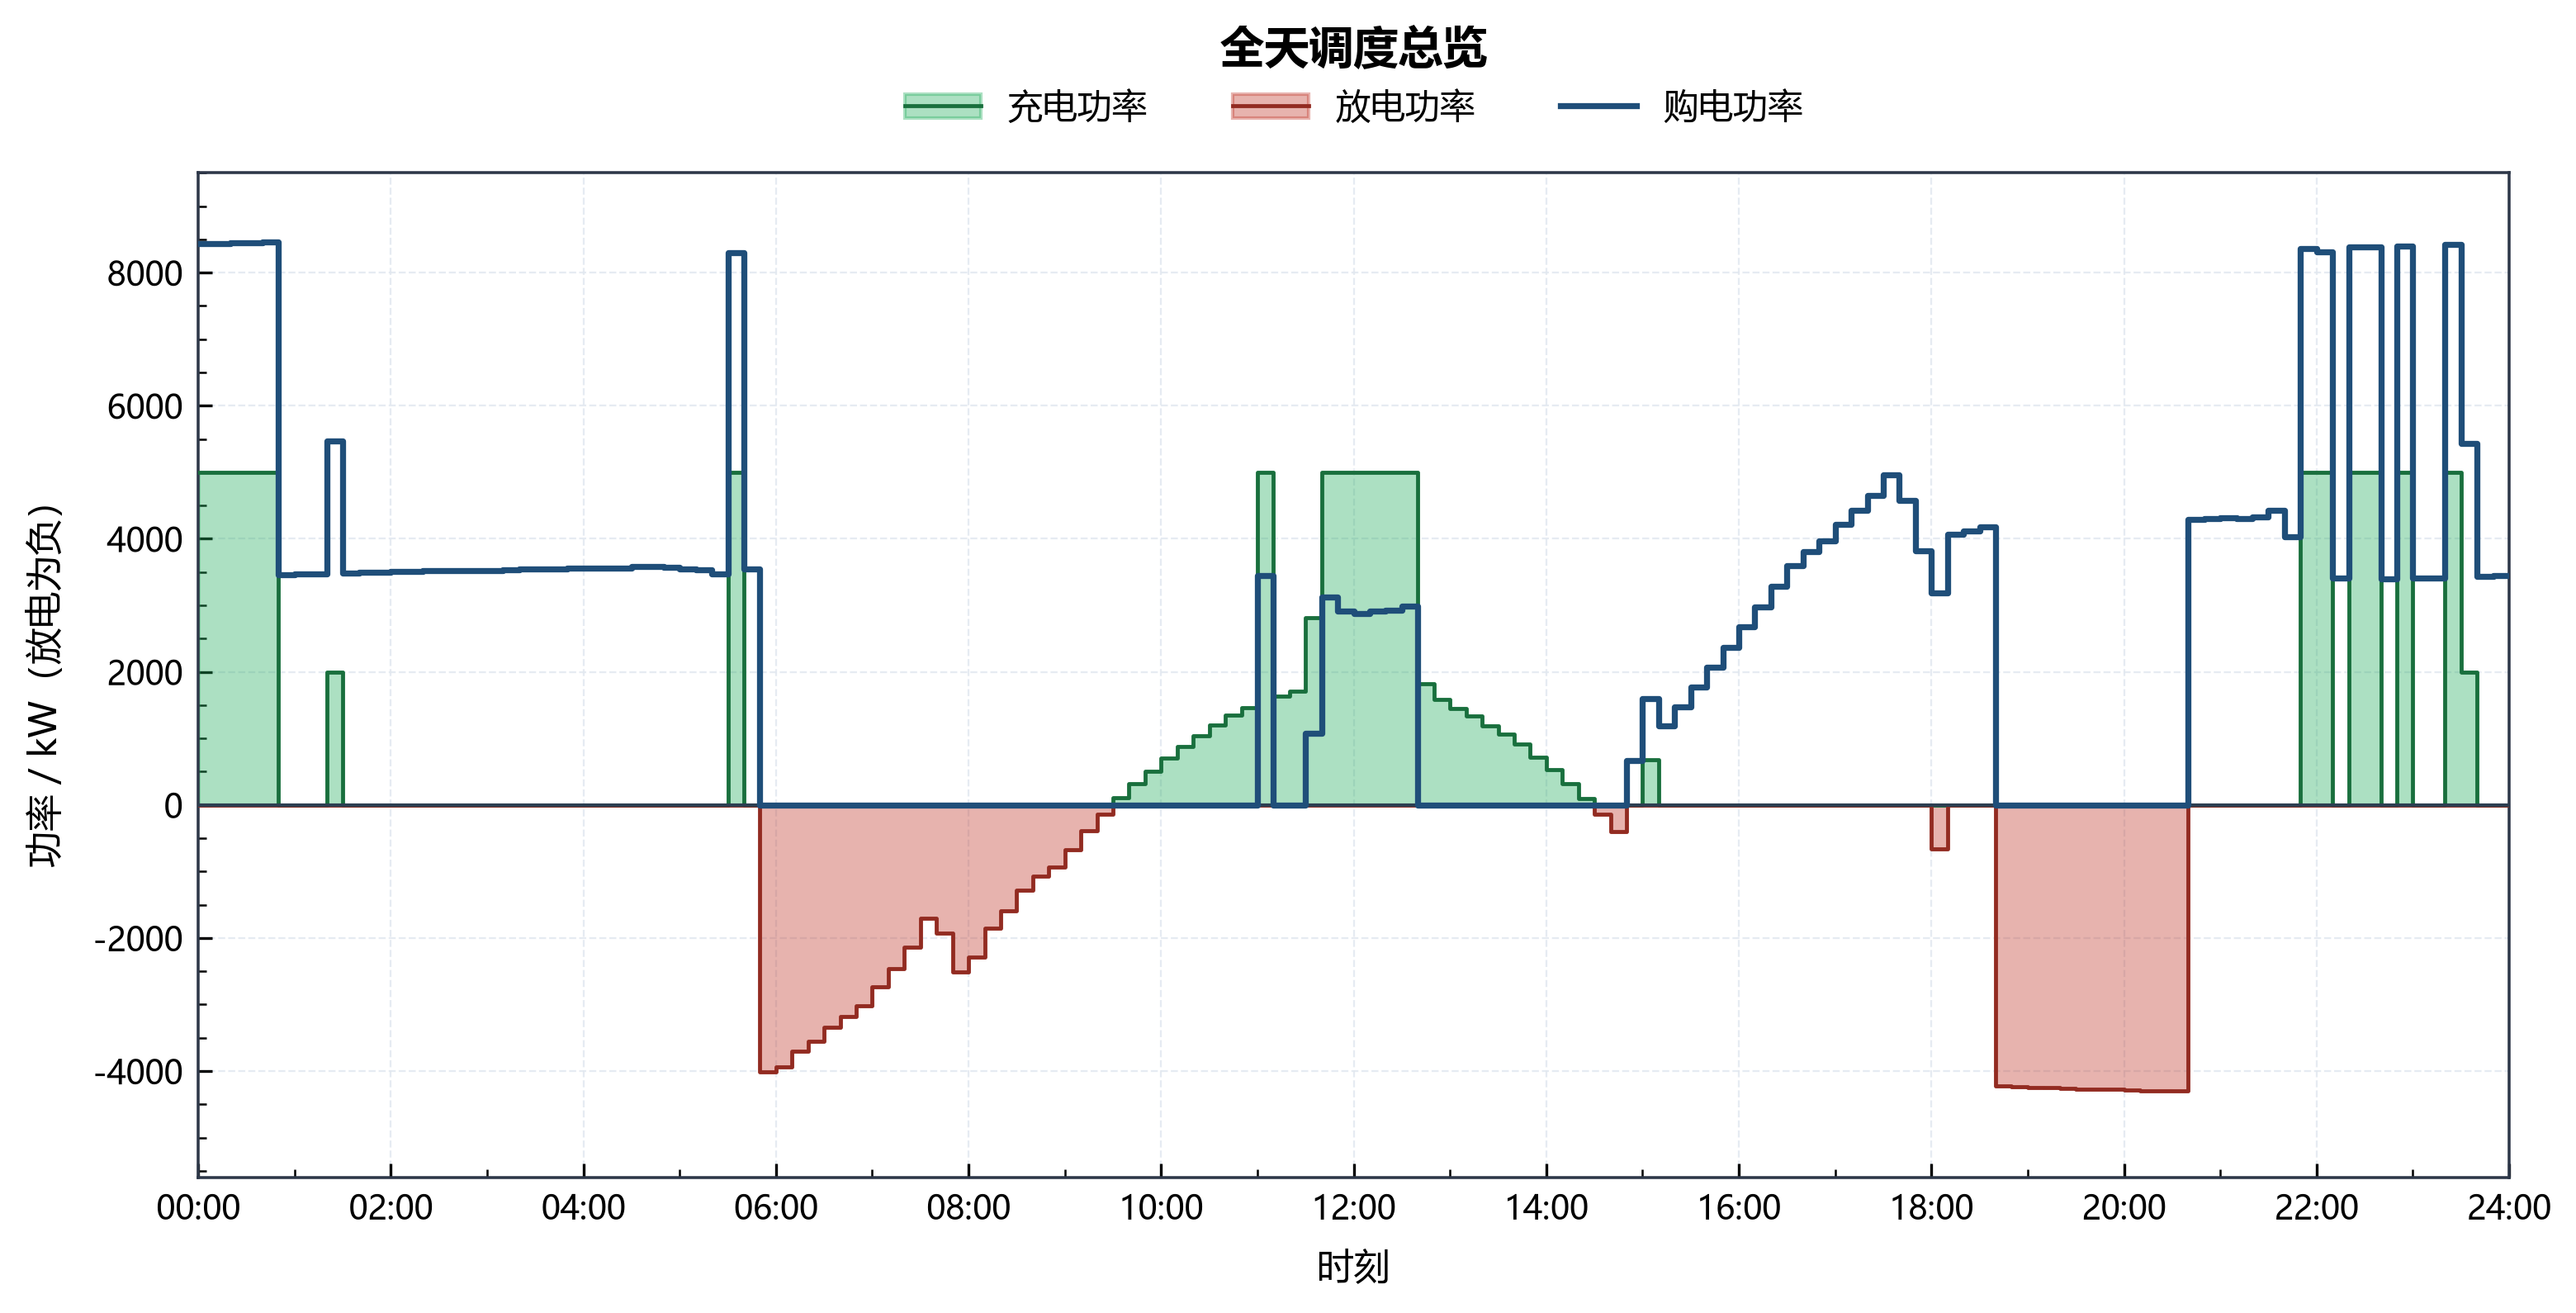
\includegraphics[width=0.92\textwidth]{../../C题/问题一可能用到的图片/全天调度总览.png}
  \caption{问题一最优调度下的全天购电、充电与放电功率}
  \label{fig:q1_dispatch_overview}
\end{figure}

\begin{figure}[H]
  \centering
  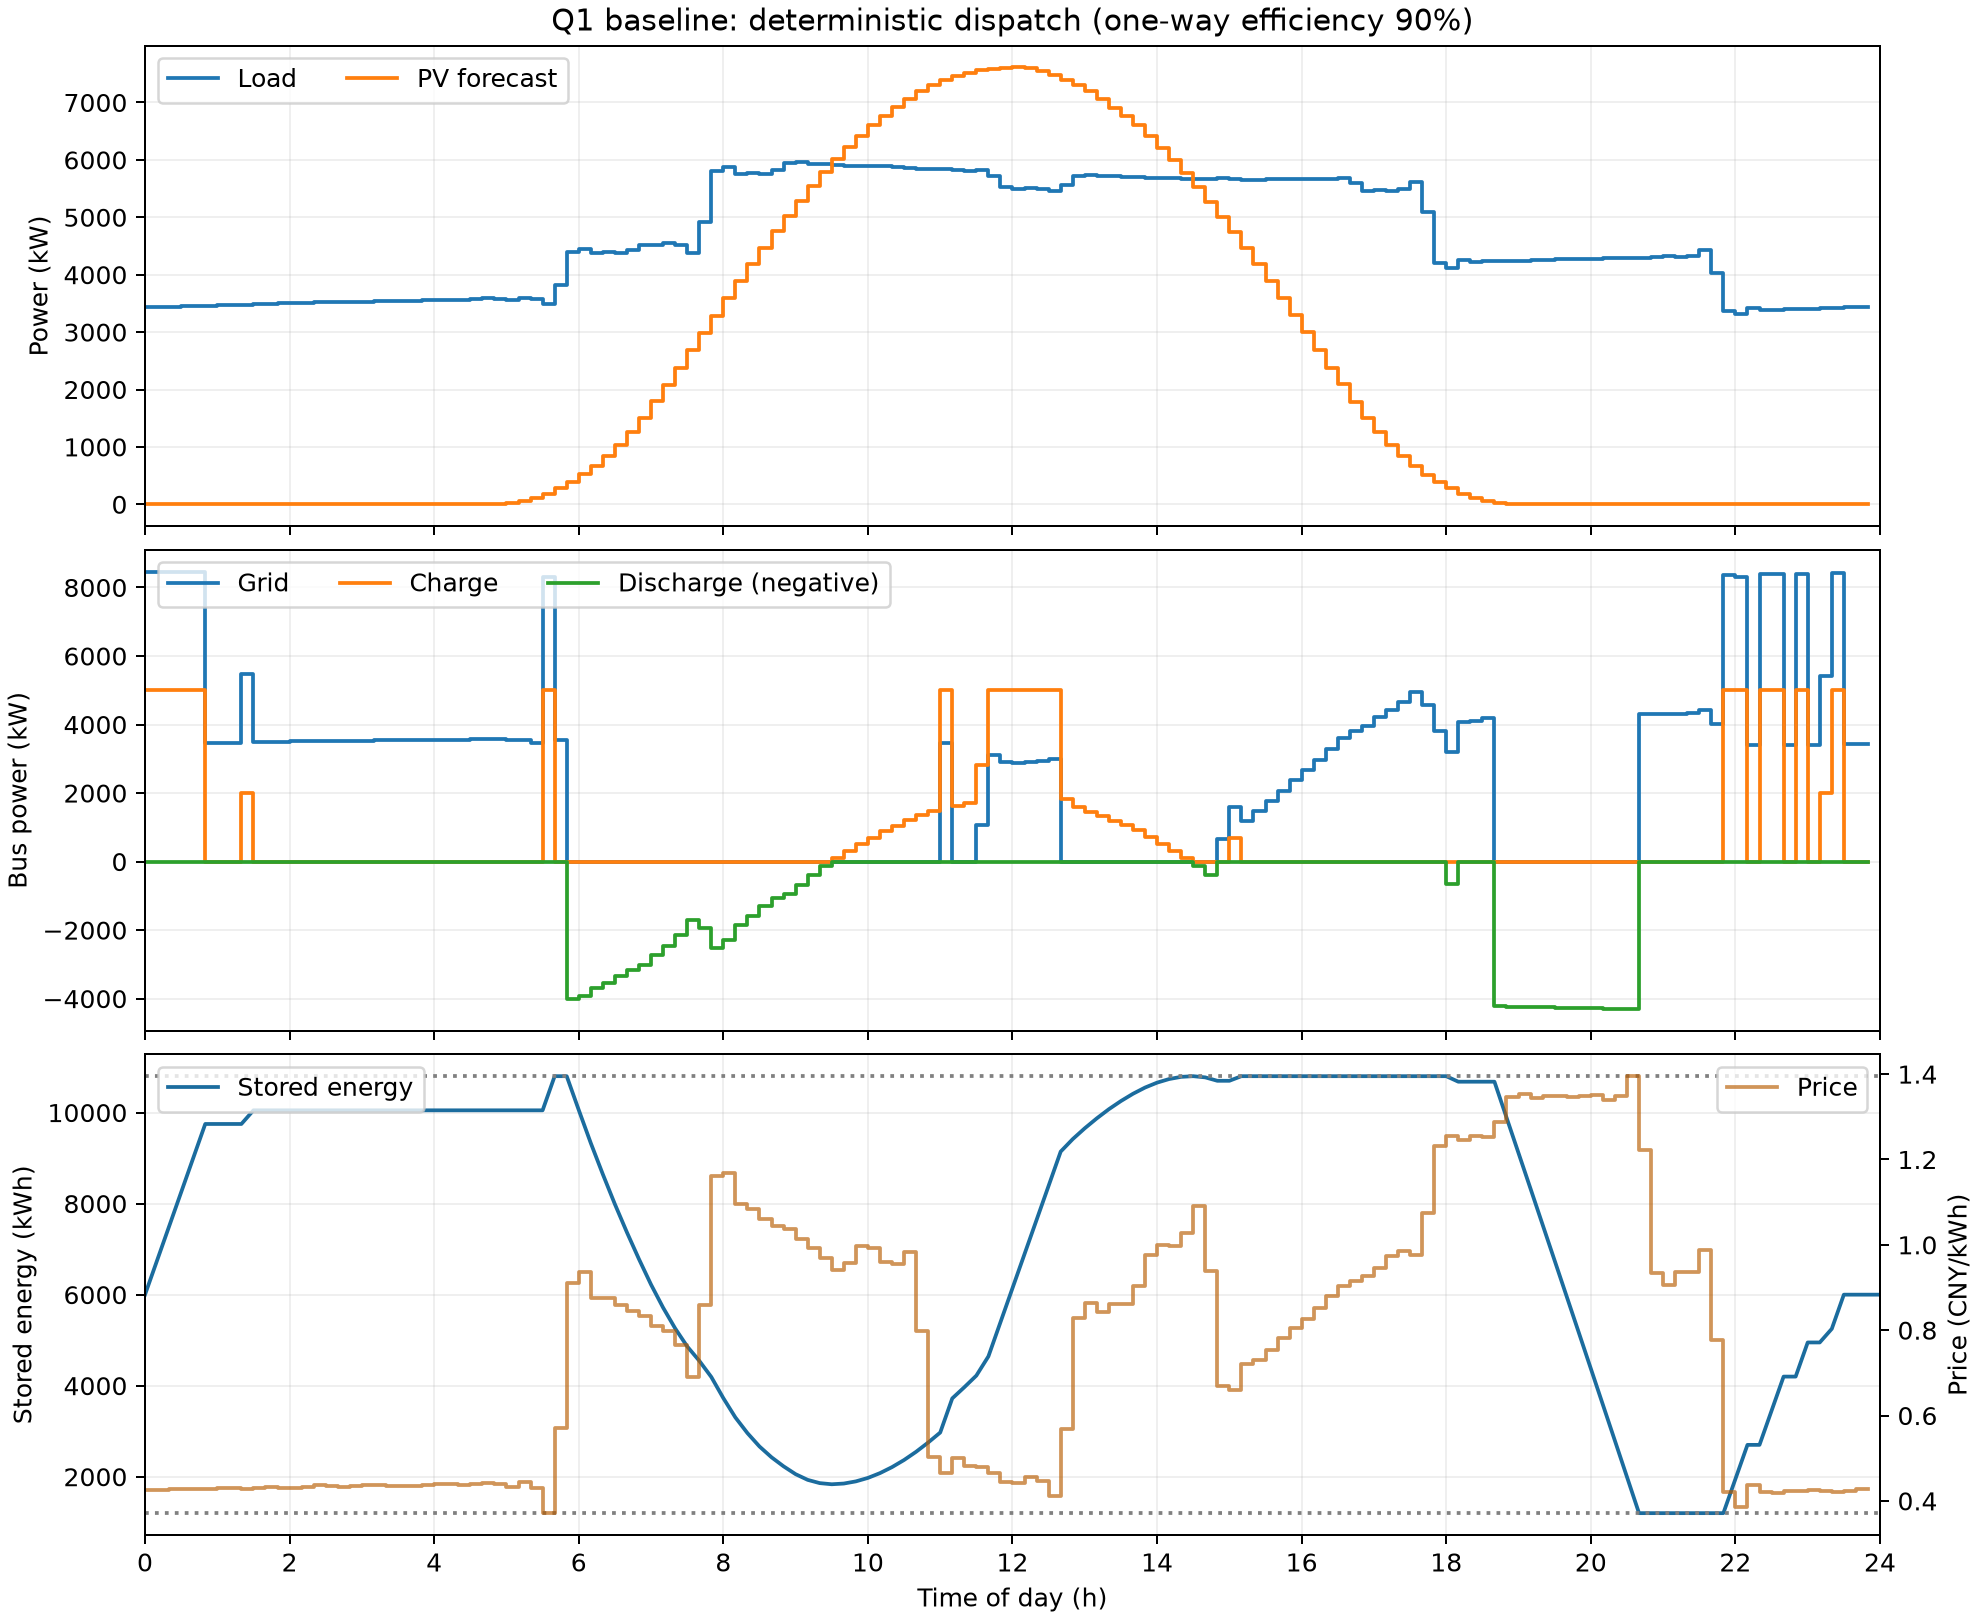
\includegraphics[width=0.92\textwidth]{../../C题/figures/q1_baseline.png}
  \caption{问题一最优调度下的负载、光伏、母线功率、储电量与电价运行曲线}
  \label{fig:q1_operation_curve}
\end{figure}

图~\ref{fig:q1_dispatch_overview}中放电功率显示为负值，表示储能向母线供电；图~\ref{fig:q1_operation_curve}中储电量始终位于$1200$--$10800$~kWh范围内，日末回到$6000$~kWh，与表~\ref{tab:q1_storage}结果一致。

\subsubsection{结果分析与验证}

\paragraph{（1）最优策略的经济学解释}

图~\ref{fig:q1_dispatch_overview}与图~\ref{fig:q1_operation_curve}所示的调度时序本质上是\textbf{通过储能设备实现电力的时间套利}：凌晨谷价时段大量购电并充电，白天光伏盈余时段停止购电，傍晚高价时段依靠储能放电覆盖负载，深夜再恢复购电补充储能。以$\eta_c \cdot \eta_d = 0.81$的往返效率为代价，低价电力被转移至高价时段使用；储能全天充电量为$20\,740.67$~kWh、放电量为$16\,799.94$~kWh，其差值$3\,940.73$~kWh即为往返能量损耗。

\paragraph{（2）与无储能方案的对比}

若不使用储能设备，当净负载为正时，微网须在每个时段直接购买等于净负载的电量。此时全天购电费用为$48\,052.05$元。最优储能调度方案的购电费用为$35\,126.95$元，\textbf{节省费用$12\,925.10$元，降幅达$26.90\%$}。这一显著的成本节约来源于储能设备对峰谷电价差的有效利用。

\paragraph{（3）LP与MILP解的对比}

为验证充放电互斥约束的必要性，本文同时求解了放松二进制变量$z_t$为连续变量$z_t \in [0, 1]$的线性规划（LP）松弛问题。结果表明：LP与MILP的最优购电费用完全相同，均为$35\,126.95$元，说明\textbf{在本实例中LP的最优解已自然满足充放电互斥条件}。

两种求解方法在144个时段中仅有2个时段的购电量存在差异（如表~\ref{tab:q1_lp_milp_diff}所示）。

\begin{table}[H]
\centering
\caption{LP与MILP求解结果的时段差异}
\label{tab:q1_lp_milp_diff}
\zihao{5}
\begin{tabular}{cccc}
\toprule
\textbf{时段} & \textbf{电价（元/kWh）} & \textbf{LP购电量（kWh）} & \textbf{MILP购电量（kWh）} \\
\midrule
$23{:}10$--$23{:}20$ & $0.4240$ & $902.69$ & $569.36$ \\
$23{:}30$--$23{:}40$ & $0.4240$ & $571.62$ & $904.95$ \\
\bottomrule
\end{tabular}
\end{table}

上述差异系等价电价时段之间充电安排的重新分配：$23{:}10$--$23{:}20$与$23{:}30$--$23{:}40$的电价均为$0.4240$~元/kWh，$333.33$~kWh的充电量在两个时段之间移动不影响总费用。这表明\textbf{最优解并非唯一}，在同一电价的相邻时段内存在调度方案的等价变换自由度。

\paragraph{（4）小结}

问题一的最优购电策略通过MILP模型精确求解，全天购电费用为$35\,126.95$元，相较于无储能方案节省$26.90\%$。最优策略的核心逻辑可以概括为"谷充峰放"——利用储能设备在低电价时段充电蓄能、在高电价时段放电供能，以最大限度地降低外购电力的综合成本。模型通过多项物理一致性校验，验证了求解结果的正确性和可靠性。


\subsection{问题二模型建立及求解}

\begin{figure}[H]
  \centering
  \includegraphics[width=0.9\textwidth]{../../C题/问题二可能用到的图片/流程图.pdf}
  \caption{问题二模型求解流程}
  \label{fig:q2_solution_flow}
\end{figure}

\subsubsection{模型建立}

\paragraph{（1）LightGBM需求预测模型}

记$k$为日期序号，在第$k$天的$0{:}00$，需利用历史数据预测当天$144$个时段的负载功率和光伏发电功率。本文采用\textbf{季节性朴素预测}方法：负载功率取$7$天前同时段的观测值，捕捉周内周期性；光伏功率取$1$天前同时段的观测值，利用相邻日的日照相似性。记第$k$天第$t$个时段的实际负载和光伏功率分别为$L_{k,t}$和$V_{k,t}$，则朴素预测值为：
\begin{equation}
  \widehat{L}_{k,t} = \begin{cases} L_{k-7,t}, & k \geq 7 \\ L_{k-1,t}, & 1 \leq k < 7 \end{cases}, \qquad \widehat{V}_{k,t} = V_{k-1,t}
  \label{eq:q2_forecast}
\end{equation}
\noindent 其中，历史样本不足$7$天时负载预测退化为昨日同段值。朴素预测能够稳定提供周内与日内基准，但难以捕捉天气和用能习惯的短期变化，因此本文进一步构造时间特征并采用\textbf{LightGBM}回归模型对负载与光伏预测进行修正：负载模型使用$15$个特征，光伏模型使用$12$个特征，特征包括历史同段观测、相邻时段观测与日内周期项，所有特征均只使用决策时刻之前已到达的数据。经修正后的预测仍记为$\widehat{L}_{k,t}$和$\widehat{V}_{k,t}$，其预测的净需求电量为：
\begin{equation}
  \widehat{n}_{k,t} = (\widehat{L}_{k,t} - \widehat{V}_{k,t}) \cdot \Delta t
  \label{eq:q2_net_demand_forecast}
\end{equation}

由于紧急购电按$5$倍电价计费，代价远高于计划购电，需对净需求预测进行上行修正。本文基于\textbf{报童模型}的最优分位数理论推导保护水平。

在无储能、单时段的简化情形下，设计划购电量为$q$，随机净需求为$X$，则期望费用为：
\begin{equation}
  f(q) = p \cdot q + 5p \cdot \mathbb{E}[(X - q)^+]
  \label{eq:q2_newsvendor}
\end{equation}
\noindent 其中$p$为电价，$(X - q)^+$为缺口部分。对连续分布取一阶条件$f'(q^*) = 0$，可得最优分位水平：
\begin{equation}
  F_X(q^*) = 1 - \frac{1}{5} = 0.8
  \label{eq:q2_optimal_quantile}
\end{equation}

\noindent 这意味着最优计划购电量应设在净需求分布的$80\%$分位数处。虽然该结论严格成立的条件是无储能的单时段情形，但将其作为含储能系统的启发式保护水平仍具有合理性。

具体实现中，定义第$j$天第$t$个时段的预测残差为$\varepsilon_{j,t} = n_{j,t} - \widehat{n}_{j,t}$。第$k$天的$0{:}00$，取最近$W = 28$天的历史残差集合$\mathcal{H}_k = \{j: \max(1, k-28) \leq j < k\}$，样本数$m = |\mathcal{H}_k|$，计算每个时段的经验$80\%$分位数修正量：
\begin{equation}
  r_{k,t} = \begin{cases} \varepsilon_{(\lceil 0.8m \rceil), t}, & m \geq 7 \\ 0, & m < 7 \end{cases}
  \label{eq:q2_quantile_correction}
\end{equation}
\noindent 其中$\varepsilon_{(\lceil 0.8m \rceil), t}$为将$\mathcal{H}_k$中第$t$个时段的残差升序排列后的第$\lceil 0.8m \rceil$个值。修正后的保护性净需求为：
\begin{equation}
  \widetilde{n}_{k,t} = \widehat{n}_{k,t} + r_{k,t}
  \label{eq:q2_protected_demand}
\end{equation}

\paragraph{（2）日前购电计划MILP模型}

将修正后的保护性净需求$\widetilde{n}_{k,t}$代入问题一的MILP框架。与问题一的差异在于：日初储电量$E_{k,0}$由前一日实际运行的末态储电量跨日继承，不再固定为$6\,000$~kWh；名义计划不施加固定日末电量，仅保留储电量上下界，以避免人为规定日末库存造成购电扭曲。新时间口径下，自由名义末态较固定$6\,000$~kWh名义末态全期节省$28\,710.48$元，因此问题二正式方案采用自由名义末态，实际储电量由运行轨迹跨日继承。

日前MILP模型为：
\begin{equation}
\begin{aligned}
  & \boxed{\min \quad \sum_{t=0}^{143} p_t \cdot q_{k,t}} \\
  & \text{s.t.} \quad q_{k,t} + \bar{d}_{k,t} = \widetilde{n}_{k,t} + \bar{c}_{k,t} + \bar{w}_{k,t}, \\
  & \quad\quad\; \bar{E}_{k,t+1} = \bar{E}_{k,t} + \eta_c \bar{c}_{k,t} - \bar{d}_{k,t}/\eta_d, \\
  & \quad\quad\; E_{\min} \leq \bar{E}_{k,t} \leq E_{\max}, \\
  & \quad\quad\; 0 \leq \bar{c}_{k,t} \leq M \bar{z}_{k,t}, \; 0 \leq \bar{d}_{k,t} \leq M(1-\bar{z}_{k,t}), \\
  & \quad\quad\; \bar{E}_{k,0} = E_{k,0} \\
  & \quad\quad\; q_{k,t}, \bar{w}_{k,t} \geq 0, \quad \bar{z}_{k,t} \in \{0,1\}
\end{aligned}
\label{eq:q2_milp}
\end{equation}

\noindent 其中除储电量界对$t=0,1,\ldots,144$成立外，其余约束均对$t=0,1,\ldots,143$成立。

\noindent 求解得到的$q_{k,t}$在$0{:}00$冻结为当天的计划购电量。名义充放电$\bar{c}_{k,t}$、$\bar{d}_{k,t}$仅用于保证计划可行性，\textbf{实际充放电由下述反馈机制确定}。

\paragraph{（3）实际储能反馈与费用核算模型}

当天实际供需按时段逐步揭示。定义第$t$个时段的供需盈余为$s_t = q_{k,t} - n_{k,t}$，其中$n_{k,t} = (L_{k,t} - V_{k,t}) \cdot \Delta t$为实际净需求。储能设备按如下贪心规则运行：

\textbf{情形一：供给盈余，即$s_t \geq 0$}——优先为储能充电：
\begin{equation}
  c_t = \min\{s_t,\; M,\; (E_{\max} - E_t)/\eta_c\}, \quad d_t = e_t = 0, \quad w_t = s_t - c_t
  \label{eq:q2_surplus}
\end{equation}

\textbf{情形二：供给不足，即$s_t < 0$}——优先由储能放电补缺：
\begin{equation}
  d_t = \min\{-s_t,\; M,\; \eta_d(E_t - E_{\min})\}, \quad e_t = -s_t - d_t, \quad c_t = w_t = 0
  \label{eq:q2_deficit}
\end{equation}
\noindent 其中$e_t$为紧急购电量。储电量按$E_{t+1} = E_t + \eta_c c_t - d_t/\eta_d$更新，日末实际储电量$E_{k,144}$直接继承为次日日初储电量$E_{k+1,0}$。

全期指$2025$年$2$月至$12$月共$334$天，总购电费用为：
\begin{equation}
  C = \sum_{k \in \mathcal{K}} \sum_{t=0}^{143} \left( p_t \cdot q_{k,t} + 5 p_t \cdot e_{k,t} \right)
  \label{eq:q2_total_cost}
\end{equation}
\noindent 其中计划购电全额付费，无论是否使用均按计划量计费；紧急购电按$5$倍电价计费。

\subsubsection{模型求解}

\noindent\textbf{（1）求解流程}\\[6pt]

\step{1} \textbf{公共预运行} 以$2025$年$1$月$1$日$0{:}00$初始储电量$E_0 = 6\,000$~kWh为起点，运行$1$月$31$天形成预测残差历史并递推储能状态，得到$2$月$1$日日初实际储电量为$6\,075.80$~kWh。$1$月不计入正式评价费用。

\step{2} \textbf{逐日滚动优化} 从$2$月$1$日起，每个自然日在$0{:}00$生成当天$144$个时段的负载与光伏预测，计算历史残差的$q_{80}$修正量得到保护性净需求，求解日前MILP模型后将计划购电量冻结为当天的执行依据。

\step{3} \textbf{逐段实际执行} 按式~\eqref{eq:q2_surplus}--\eqref{eq:q2_deficit}逐段反馈执行，记录充放电量、紧急购电量和储电量。

\step{4} \textbf{日末状态继承} 实际日末储电量继承为次日日初储电量，滚动推进至$12$月$31$日。

\paragraph{（2）名义末态对照实验}

为检验名义末态设置的稳健性，本文在新时间口径下分别求解固定$6\,000$~kWh名义末态与自由名义末态两组方案，如表~\ref{tab:q2_ablation}所示。固定组全期总费用为$13\,728\,048.17$元，自由组为$13\,699\,337.68$元，自由组少$28\,710.48$元，降幅为$0.2091\%$，且在$11/11$个月中均更省；自由组应急电量增加$4\,754$~kWh、期末储电量为$1\,682.90$~kWh，说明其节费来自更灵活地利用本日购电与跨日库存，而非抬高期末借用量。因此，问题二正式方案采用自由名义末态。

\begin{table}[H]
\centering
\caption{问题二名义末态对照：$2$--$12$月总费用对比}
\label{tab:q2_ablation}
\zihao{5}
\resizebox{\textwidth}{!}{%
\begin{tabular}{cccccc}
\toprule
\textbf{方案} & \textbf{名义末态} & \textbf{总费用（元）} & \textbf{计划购电费（元）} & \textbf{应急费（元）} & \textbf{期末储电（kWh）} \\
\midrule
$N_{\text{fixed}}$ & 固定$6\,000$~kWh   & $13\,728\,048.17$ & $13\,303\,179.06$ & $424\,869.11$ & $6\,287.69$ \\
$N_{\text{free}}$  & 自由末态           & $\bm{13\,699\,337.68}$ & $13\,264\,904.28$ & $434\,433.41$ & $1\,682.90$ \\
\bottomrule
\end{tabular}}
\end{table}

\subsubsection{结果展示}

\paragraph{（1）全期关键指标}

\begin{table}[H]
\centering
\caption{问题二正式方案在LightGBM预测、q80残差保护与自由名义末态下的全期运行指标}
\label{tab:q2_summary}
\zihao{5}
\begin{tabular}{lc}
\toprule
\textbf{指标} & \textbf{数值} \\
\midrule
计划购电费（元）    & $13\,264\,904.28$ \\
紧急购电费（元）    & $434\,433.41$ \\
总费用（元）        & $13\,699\,337.68$ \\
计划购电量（kWh）   & $21\,635\,744.29$ \\
紧急购电量（kWh）   & $73\,095.96$ \\
未使用电量（kWh）   & $2\,573\,521.97$ \\
全期充电量（kWh）   & $6\,317\,463.66$ \\
全期放电量（kWh）   & $5\,121\,099.18$ \\
全期损耗（kWh）     & $1\,200\,757.39$ \\
紧急购电天数        & $119$ / $334$天 \\
紧急购电时段数      & $577$ / $48\,096$段 \\
紧急购电事件数      & $218$ \\
日初储电量（$2$月$1$日） & $6\,075.80$~kWh \\
日末储电量（$12$月$31$日） & $1\,682.90$~kWh \\
\bottomrule
\end{tabular}
\end{table}

图~\ref{fig:q2_annual_cost}给出问题二全年费用构成与应急购电占比，计划购电费与应急购电费分别占总费用的$96.83\%$和$3.17\%$，应急购电保持较低水平。

\begin{figure}[H]
  \centering
  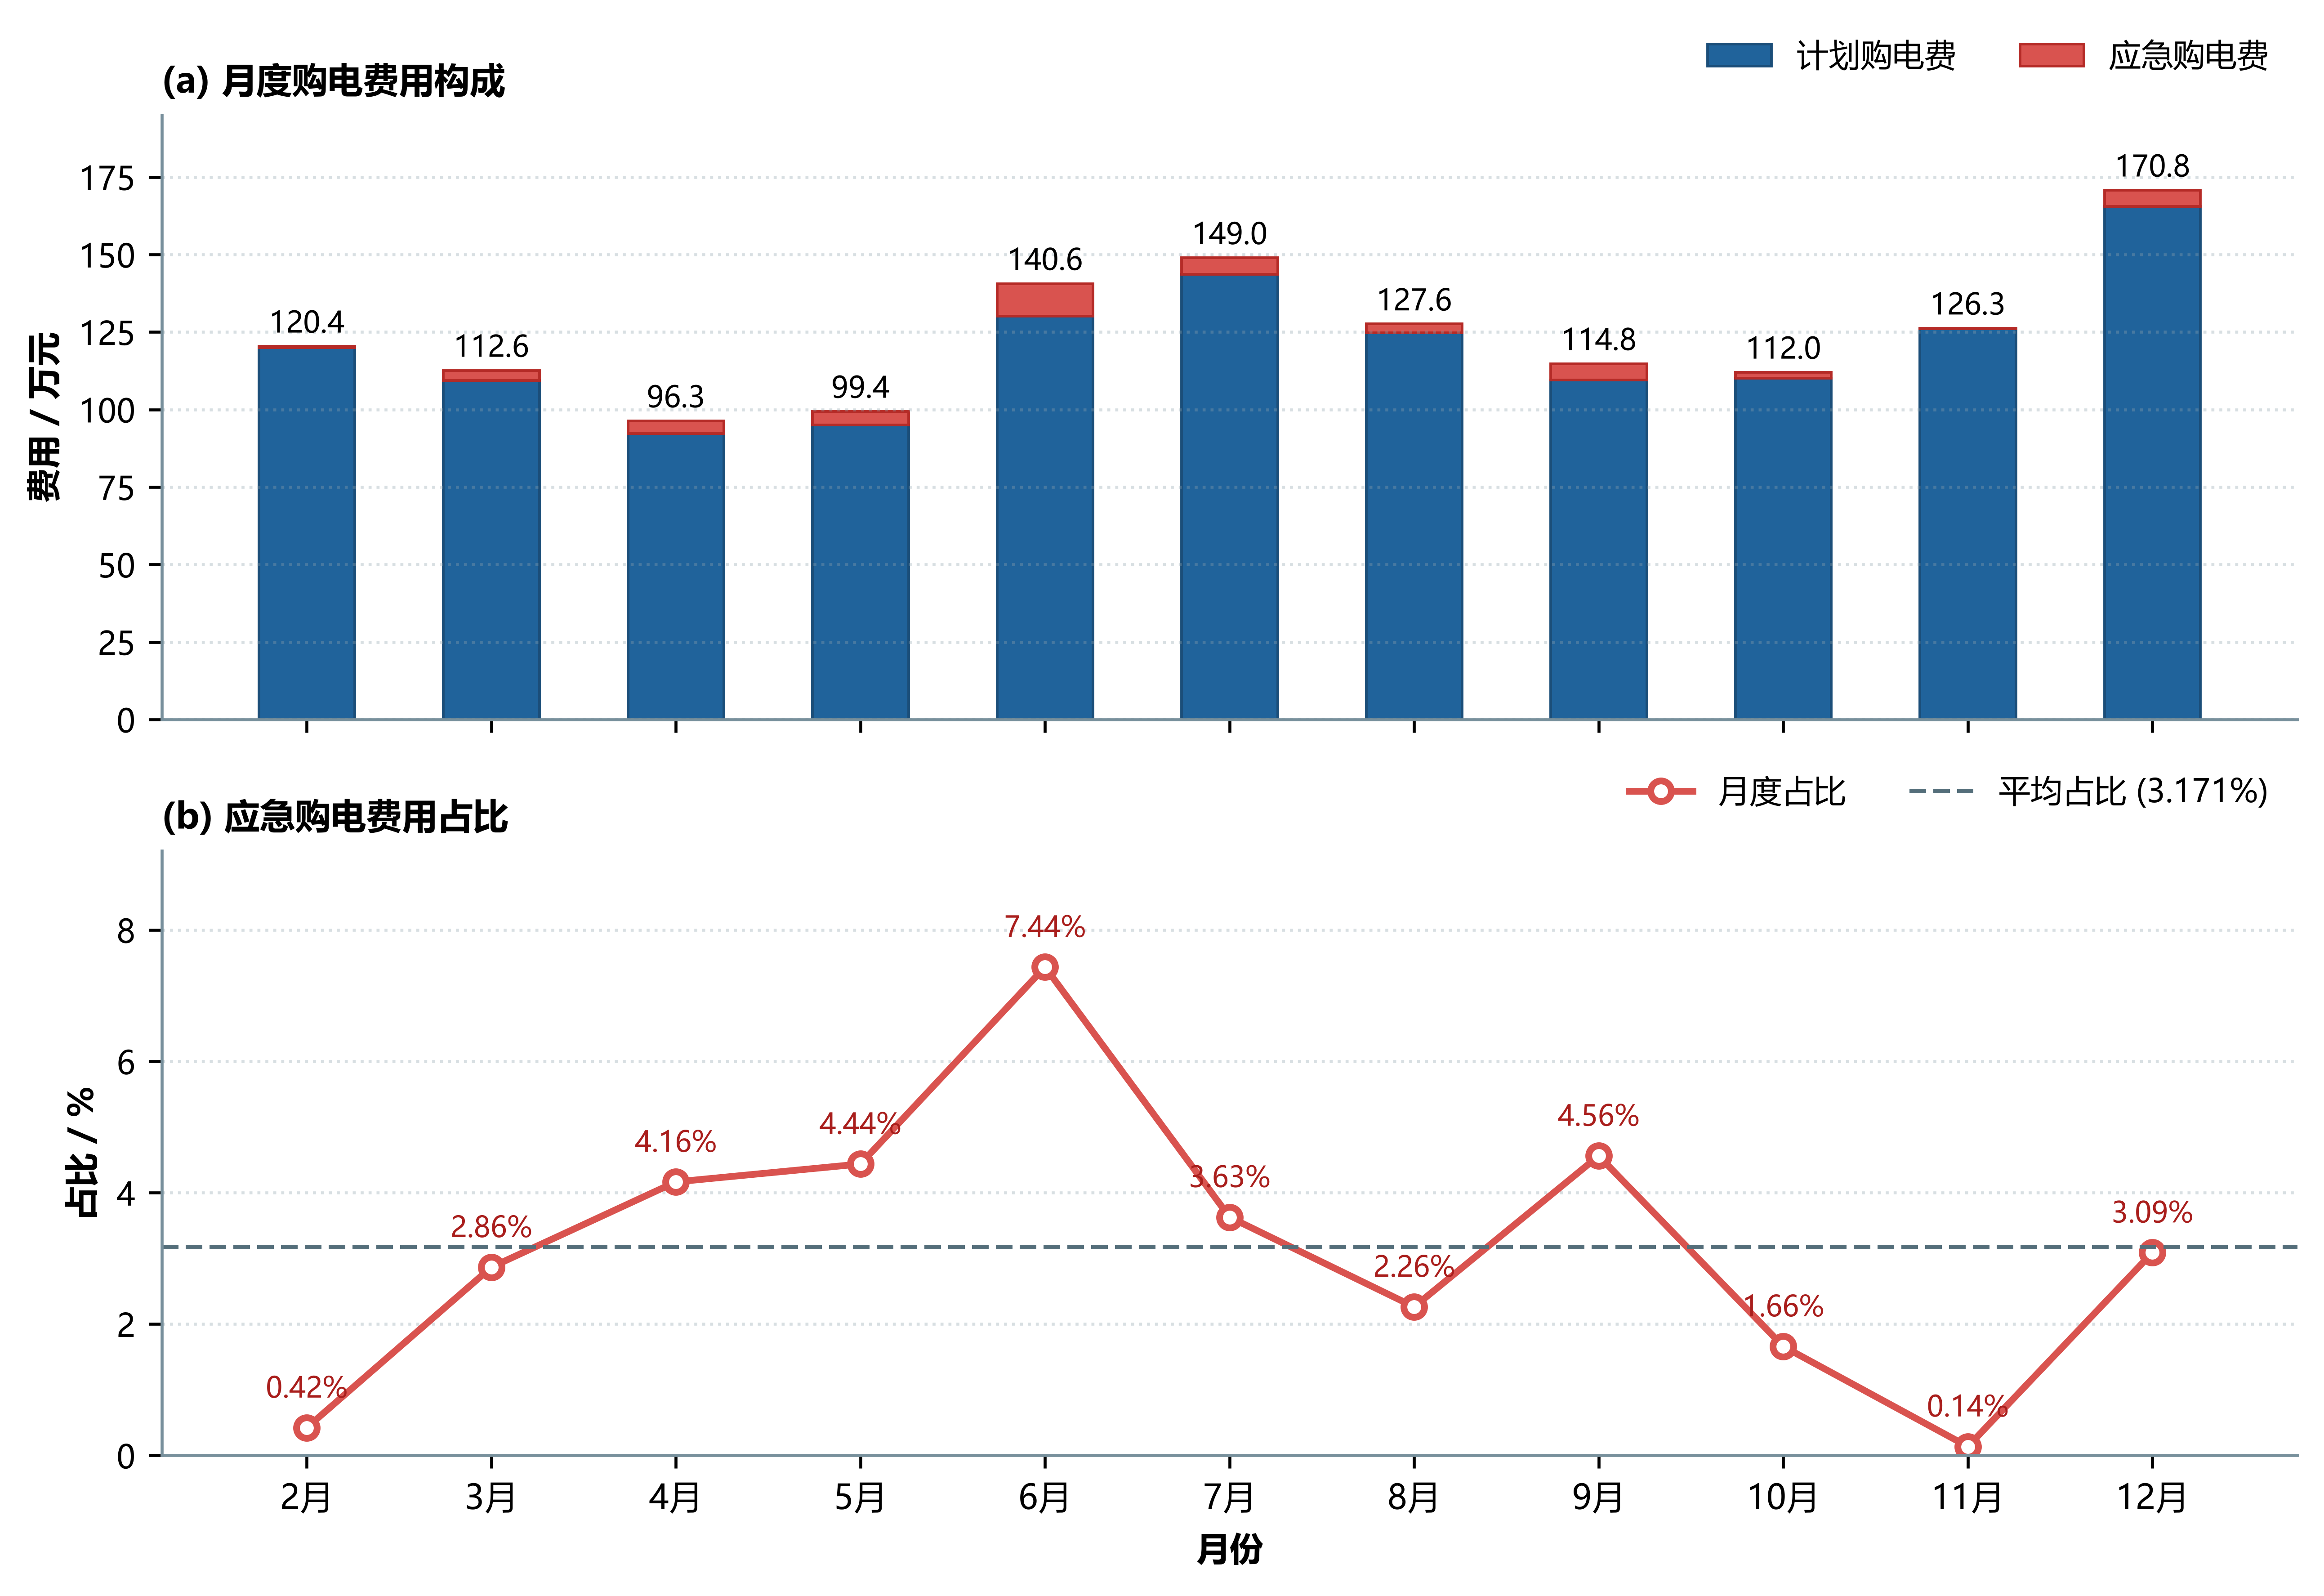
\includegraphics[width=0.88\textwidth]{../../C题/问题二可能用到的图片/q2_fig1_annual_cost_and_emergency_share.png}
  \caption{问题二全年费用构成与应急购电占比}
  \label{fig:q2_annual_cost}
\end{figure}

\paragraph{（2）指定日期的计划购电结果}

按题目要求，表~\ref{tab:q2_specified_purchase}给出$4$个指定日期的指定时段购电量及全天购电量与购电费。

\begin{table}[H]
\centering
\caption{微网在指定日期指定时段的购电量及全天购电量和购电费}
\label{tab:q2_specified_purchase}
\zihao{5}
\begin{tabular}{c|cccccc|cc}
\toprule
\textbf{日期} & $10{:}00$ & $12{:}00$ & $14{:}00$ & $16{:}00$ & $18{:}00$ & $20{:}00$ & \textbf{全天购电量} & \textbf{全天总费用} \\
 & --$10{:}10$ & --$12{:}10$ & --$14{:}10$ & --$16{:}10$ & --$18{:}10$ & --$20{:}10$ & (kWh) & (元) \\
\midrule
3.20 & $0.00$ & $640.55$ & $0.00$ & $447.48$ & $736.81$ & $0.00$ & $69\,041.05$ & $42\,052.04$ \\
6.21 & $0.00$ & $0.00$ & $0.00$ & $144.98$ & $434.65$ & $0.00$ & $35\,266.62$ & $20\,595.58$ \\
9.23 & $0.00$ & $539.99$ & $0.00$ & $442.32$ & $793.44$ & $0.00$ & $68\,835.88$ & $45\,645.24$ \\
12.21 & $0.00$ & $1\,047.81$ & $0.00$ & $809.84$ & $727.88$ & $0.00$ & $97\,787.67$ & $63\,095.90$ \\
\bottomrule
\end{tabular}
\end{table}

\noindent\textit{注：全天购电量为模板$144$个时段的计划购电量合计，全天总费用为自然日账本下的普通购电费与应急购电费之和。}

\paragraph{（3）指定日期的储能充放电量}

表~\ref{tab:q2_specified_storage}给出$4$个指定日期储能设备在$6$个$4$小时时段的充放电量，以及$0{:}00$和$24{:}00$的储电量。

\begin{table}[H]
\centering
\caption{问题二指定日期储能设备前三个$4$小时时段的充放电量及首尾储电量}
\label{tab:q2_specified_storage}
\zihao{5}
\begin{tabular}{c|cc|cc|cc|cc}
\toprule
\textbf{日期} & \multicolumn{2}{c|}{$0{:}00$--$4{:}00$} & \multicolumn{2}{c|}{$4{:}00$--$8{:}00$} & \multicolumn{2}{c|}{$8{:}00$--$12{:}00$} & \multicolumn{2}{c}{$0{:}00$ / $24{:}00$储电量} \\
 & 充 & 放 & 充 & 放 & 充 & 放 & (kWh) & (kWh) \\
\midrule
3.20 & $8\,157.56$ & $68.72$ & $1\,917.10$ & $4\,624.04$ & $5\,456.09$ & $3\,265.56$ & $2\,053.71$ & $1\,635.16$ \\
6.21 & $786.89$ & $53.34$ & $1\,192.46$ & $1\,722.27$ & $9\,282.35$ & $0.00$ & $2\,637.38$ & $2\,965.10$ \\
9.23 & $9\,051.18$ & $17.69$ & $1\,564.10$ & $5\,403.13$ & $4\,627.39$ & $2\,387.94$ & $1\,420.50$ & $1\,566.48$ \\
12.21 & $8\,533.59$ & $166.44$ & $2\,389.50$ & $686.66$ & $5\,009.77$ & $7\,911.68$ & $1\,917.10$ & $1\,798.21$ \\
\bottomrule
\end{tabular}
\end{table}

\begin{table}[H]
\centering
\zihao{5}
\begin{tabular}{c|cc|cc|cc}
\toprule
\textbf{日期} & \multicolumn{2}{c|}{$12{:}00$--$16{:}00$} & \multicolumn{2}{c|}{$16{:}00$--$20{:}00$} & \multicolumn{2}{c}{$20{:}00$--$24{:}00$} \\
 & 充 & 放 & 充 & 放 & 充 & 放 \\
\midrule
3.20 & $4\,339.59$ & $363.31$ & $232.57$ & $5\,057.50$ & $521.05$ & $3\,702.95$ \\
6.21 & $0.00$ & $0.00$ & $145.88$ & $5\,016.82$ & $1\,072.58$ & $3\,021.55$ \\
9.23 & $5\,018.31$ & $549.14$ & $156.79$ & $5\,000.36$ & $522.25$ & $3\,471.77$ \\
12.21 & $7\,498.61$ & $2\,220.11$ & $16.02$ & $4\,871.82$ & $471.38$ & $3\,624.59$ \\
\bottomrule
\end{tabular}
\end{table}

\paragraph{（4）紧急购电结果}

问题二正式方案在评价期内共发生$218$起紧急购电事件，涉及$119$天、$577$个时段，总紧急购电量$73\,095.96$~kWh，紧急购电费$434\,433.41$元。紧急购电主要出现在光伏出力快速变化的早晨以及负载与光伏预测偏差叠加的傍晚至夜间时段。表~\ref{tab:q2_emergency_sample}给出指定日期的紧急购电情况。

\begin{table}[H]
\centering
\caption{问题二正式方案指定日期的紧急购电情况}
\label{tab:q2_emergency_sample}
\zihao{5}
\begin{tabular}{cccc}
\toprule
\textbf{日期} & \textbf{紧急购电时段} & \textbf{紧急购电量(kWh)} & \textbf{紧急购电费(元)} \\
\midrule
2025.3.20  & 无 & $0.00$ & $0.00$ \\
2025.6.21  & 无 & $0.00$ & $0.00$ \\
2025.9.23  & 20:30--20:50、21:00--21:10 & $409.68$ & $2\,760.91$ \\
2025.12.21 & 无 & $0.00$ & $0.00$ \\
\bottomrule
\end{tabular}
\end{table}

% 此处应插入图：全期334天逐日总费用时序图，以及紧急购电费占比的月度柱状图。

% 此处应插入图：指定日期（如3月20日）的购电量与实际负载-光伏曲线叠加图，展示预测偏差与策略响应。

\subsubsection{结果分析与验证}

\paragraph{（1）风险修正效果分析}

问题二正式方案中，计划购电费为$13\,264\,904.28$元，紧急购电费为$434\,433.41$元，仅占总费用的$3.17\%$。由于紧急购电按$5$倍电价计费，q80残差保护通过小幅提高计划购电量为系统留出应对净需求低估的余量，把高价应急控制在较低水平，验证了报童模型分位数依据在该滚动框架下仍能有效平衡保护成本与风险成本。

\paragraph{（2）名义末态敏感性分析}

自由名义末态较固定$6\,000$~kWh名义末态的全期总费用少$28\,710.48$元，降幅为$0.2091\%$，且在$11/11$个月中均更省。自由组的应急电量因减少保护性购电而增加$4\,754$~kWh，但总费用仍更低，说明名义末态设置不会翻转问题二的主要结论；本文按与实际执行一致的自由末态口径填写正式结果。

图~\ref{fig:q2_monthly_cost_diff}给出自由名义末态相对固定$6\,000$~kWh名义末态的逐月费用差额，全部$11$个月的差额均为负值，与表~\ref{tab:q2_ablation}的整体结论一致。

\begin{figure}[H]
  \centering
  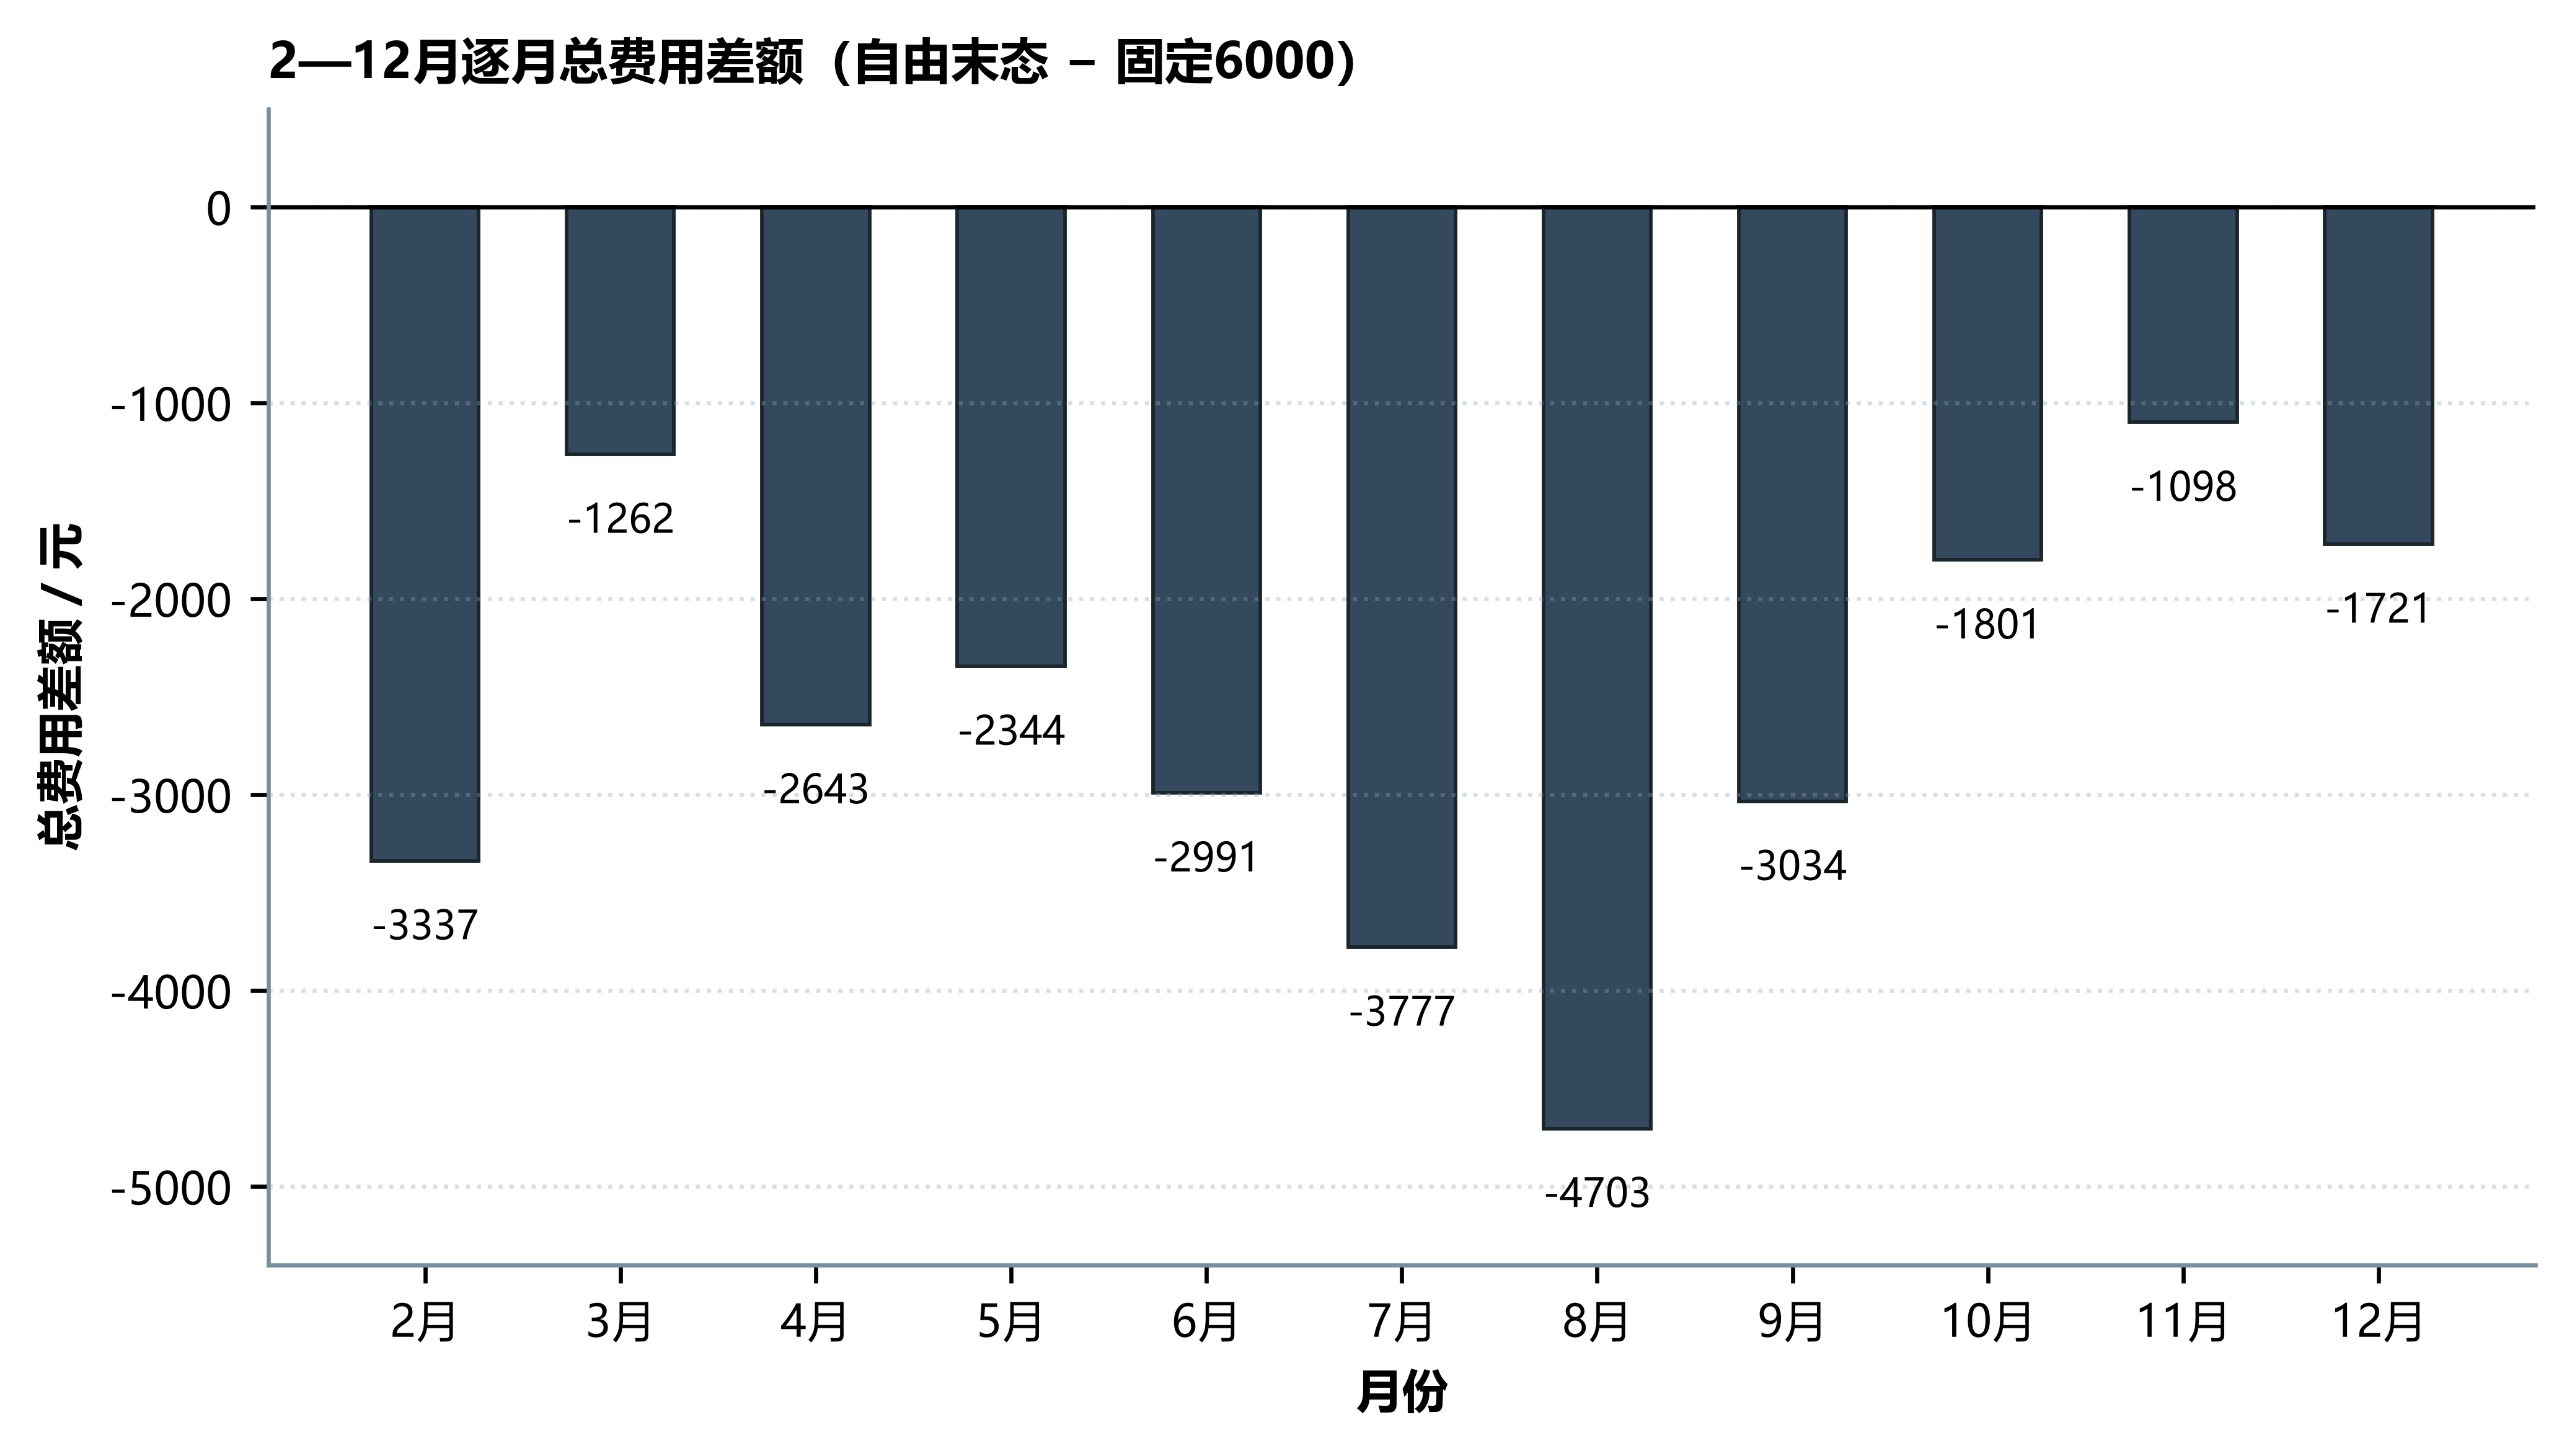
\includegraphics[width=0.88\textwidth]{../../C题/问题二可能用到的图片/q2_fig4_monthly_cost_differences.png}
  \caption{自由名义末态相对固定$6\,000$~kWh名义末态的逐月费用差额}
  \label{fig:q2_monthly_cost_diff}
\end{figure}

\paragraph{（3）物理一致性校验}

所有$334$天的逐段调度结果均通过以下检验：母线能量平衡残差、储电量递推残差、储电量边界违反量、充放电功率与互斥约束违反量等均不超过$10^{-6}$~kWh，核账误差低于$10^{-4}$元，验证了全年滚动优化的数值可靠性。

\paragraph{（4）小结}

问题二在不确定性环境下，通过"LightGBM预测$+$q80历史残差保护$+$自由名义末态MILP$+$贪心储能反馈"的四模块联合框架，实现了全期总费用$13\,699\,337.68$元，较固定名义末态方案节省$0.2091\%$，紧急购电费占比仅为$3.17\%$。该框架的核心优势在于：报童模型最优分位数理论提供了保护水平的经济学依据，自由名义末态避免了对日末库存的人为规定，贪心反馈机制保证了实际运行的物理可行性。

\subsection{问题三模型建立及求解}

\begin{figure}[H]
  \centering
  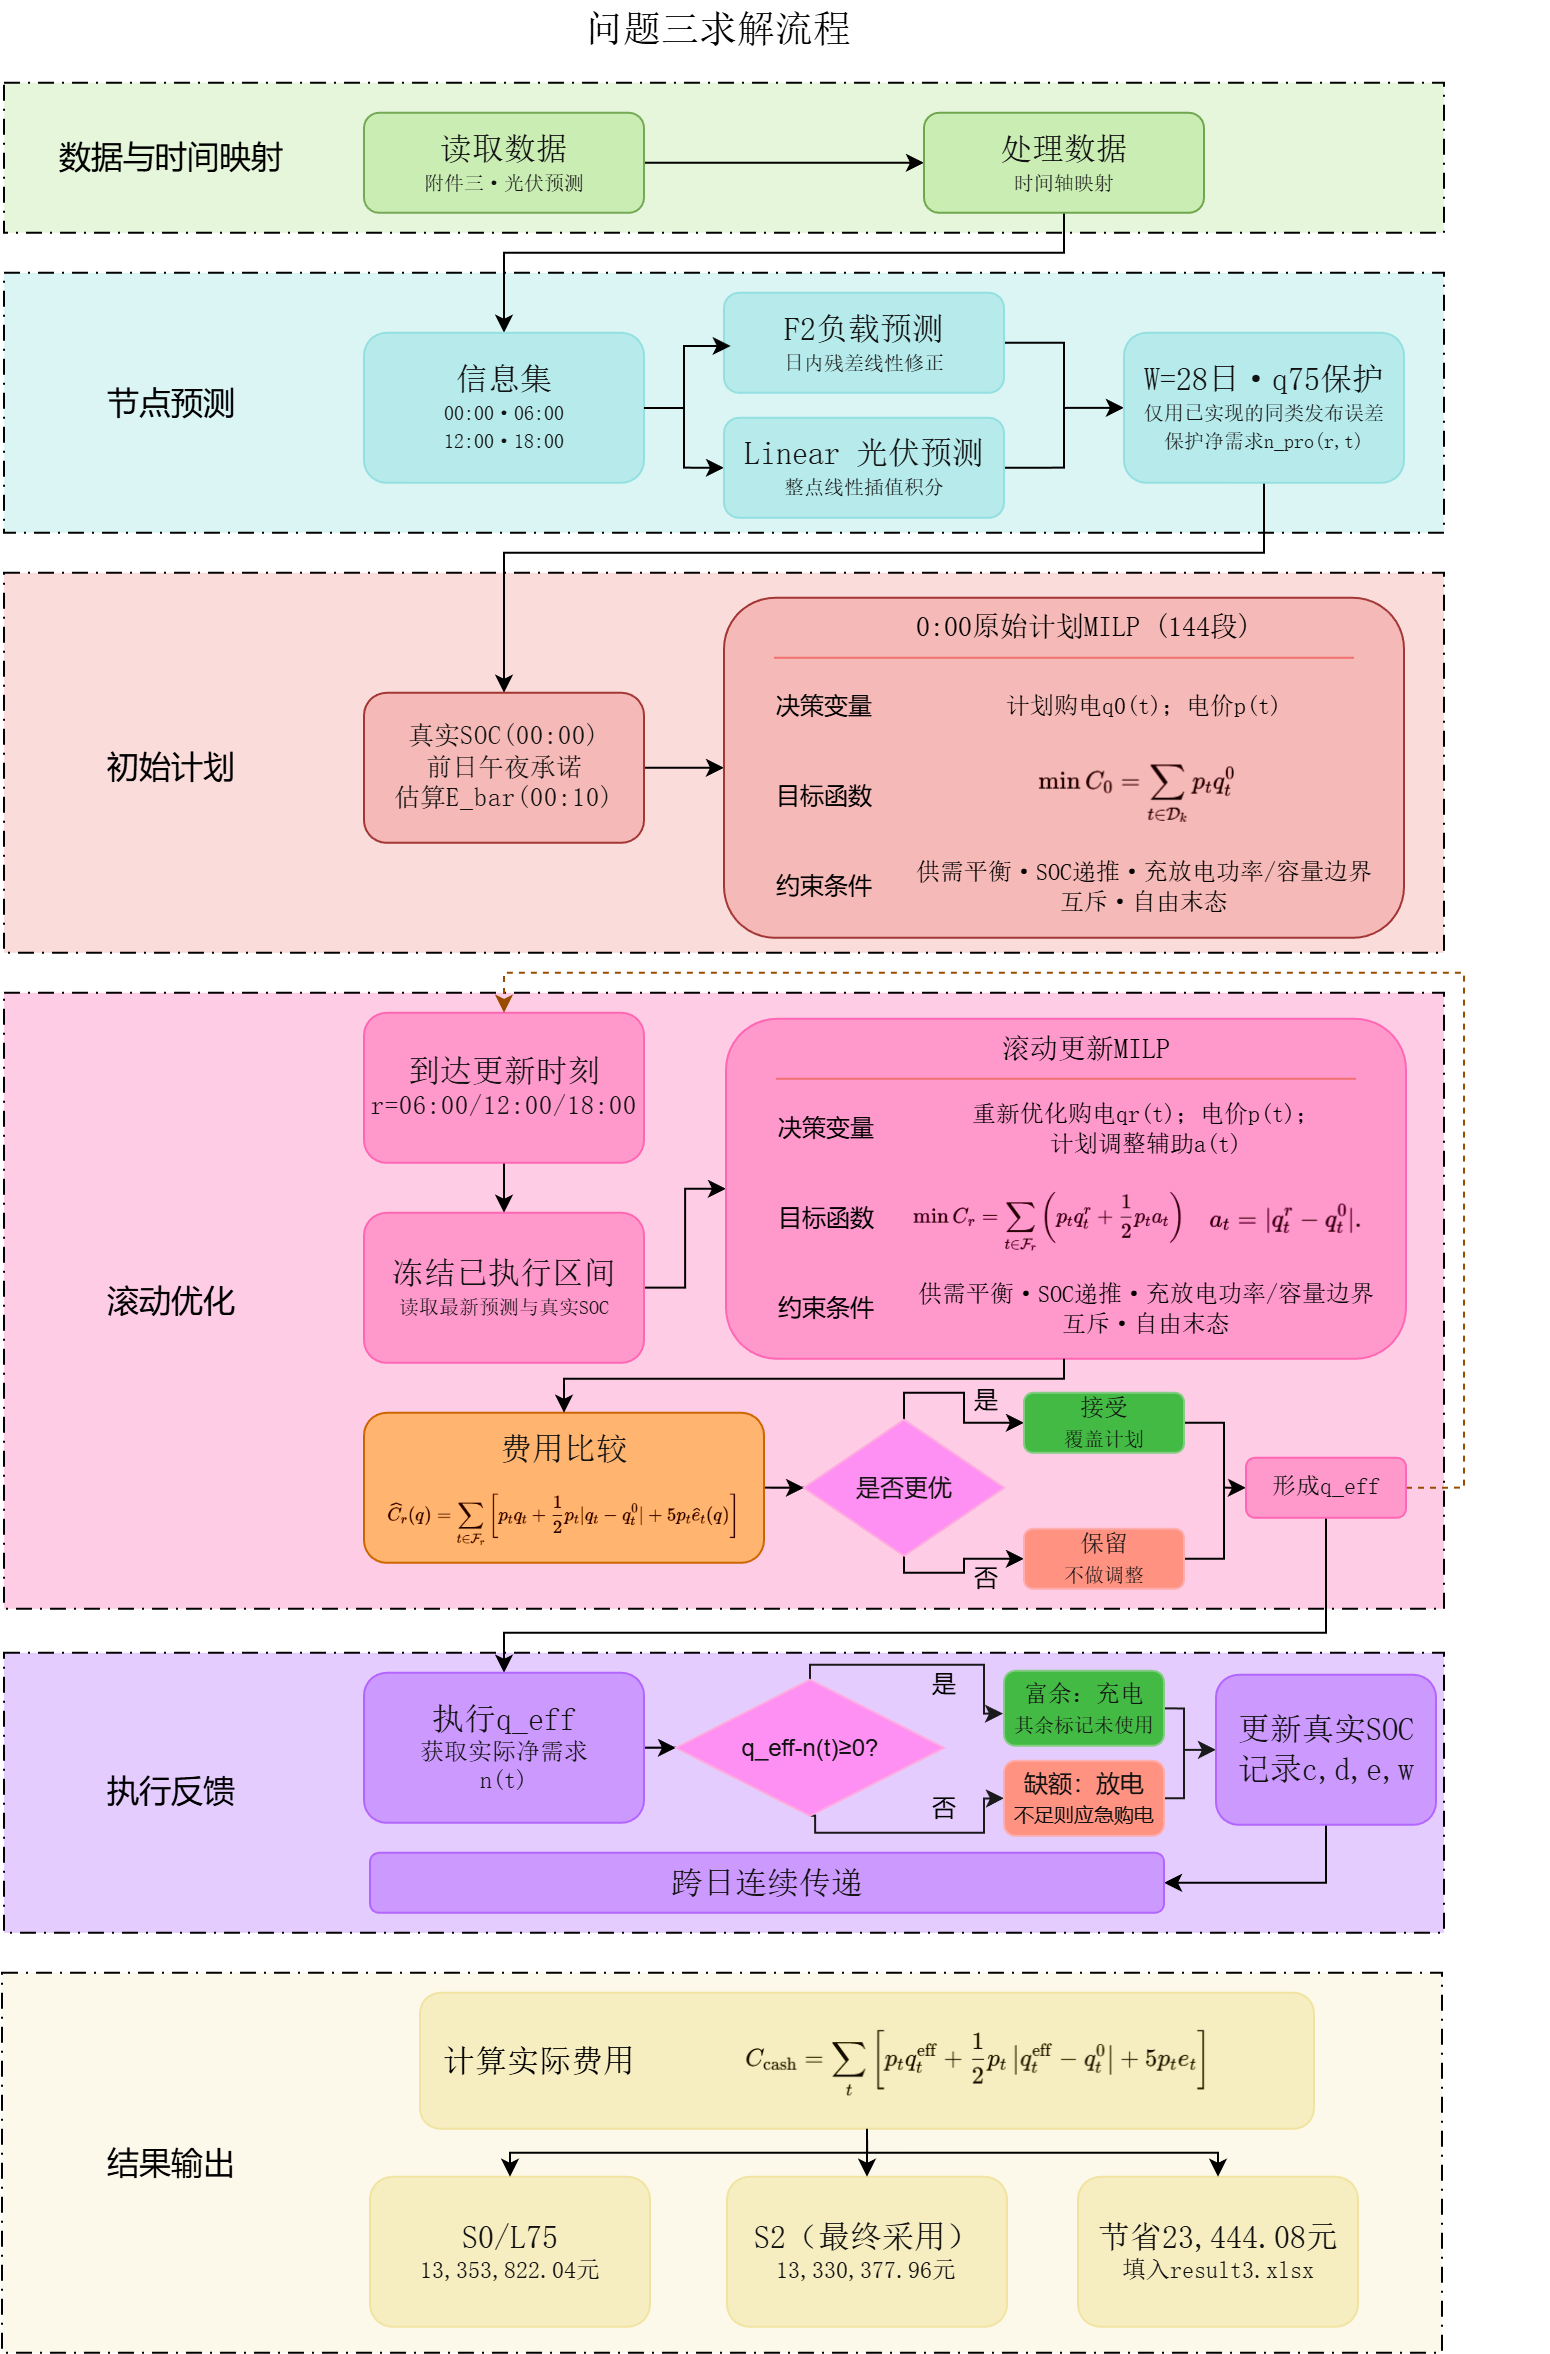
\includegraphics[width=0.9\textwidth]{../../C题/问题三可能用到的图片/流程图3.drawio.png}
  \caption{问题三模型求解流程}
  \label{fig:q3_solution_flow}
\end{figure}

\subsubsection{数据预处理}

附件3记录了$2025$年每天$0{:}00$、$6{:}00$、$12{:}00$和$18{:}00$发布的未来$24$小时整点光伏发电功率预报。由于微网调度与费用结算均在$10$分钟粒度上进行，本文先为每个发布版本独立保存发布时间、目标时刻与预测功率，不对旧版本做覆盖。对相邻整点预测功率$F_h$与$F_{h+1}$，小时内的功率采用分段线性插值：
\begin{equation}
  \widehat{V}(\tau) = (1-\theta)F_h + \theta F_{h+1}, \qquad \theta = \tau - h
  \label{eq:q3_linear_interp}
\end{equation}
\noindent 对$10$分钟区间$[t,t+\Delta t)$，以两端点预测功率的平均值作为区间代表值，并乘以时段长度得到预测电量：
\begin{equation}
  \overline{V}_t = \frac{\widehat{V}(t) + \widehat{V}(t+\Delta t)}{2}, \qquad
  \widehat{G}_t = \overline{V}_t \Delta t, \qquad \Delta t = \frac{1}{6}\ \mathrm{h}
  \label{eq:q3_interval_energy}
\end{equation}
\noindent 该变换对线性插值曲线是精确的，能够在不改变小时电量的前提下生成逐段预测值。按已确认口径，第$k$日$0{:}00$计划覆盖当日$00{:}10$至次日$00{:}10$的$144$段，$00{:}00$--$00{:}10$由前一日计划承诺执行；$6{:}00$、$12{:}00$、$18{:}00$分别调整当日剩余$109$、$73$、$37$段，优化终点均为次日$00{:}10$。首小时左端点使用发布时刻之前已可得的旧版本锚点，初始无历史版本时使用本版本首个整点值，整个过程不使用未来实测数据。

问题三沿用问题二的$W=28$日滑动窗口与$q_{80}$历史残差保护，但残差按"发布小时--目标时段"分组，避免不同发布版本的误差分布相互混合。对当前发布时刻$r$与目标区间$t$，定义预测净需求、预测残差与保护性净需求：
\begin{equation}
  \widehat{n}_{r,t} = (\widehat{L}_{r,t} - \widehat{V}_{r,t})\Delta t, \qquad
  \varepsilon_{r,t} = n_t - \widehat{n}_{r,t}, \qquad
  \widetilde{n}_{r,t} = \widehat{n}_{r,t} + \rho_{r,t}
  \label{eq:q3_protected}
\end{equation}
\noindent 其中$\widehat{L}_{r,t}$沿用问题二的$15$特征LightGBM负载预测，$n_t=(L_t-V_t)\Delta t$为实际净需求。对每组样本取此前$28$个发布日内已实现的残差，有效样本数$m\geq7$时取升序第$\lceil0.8m\rceil$个残差作为$\rho_{r,t}$，样本不足$7$个时回退零修正。该规则与问题二保持一致，作为第三问的匹配基准，不将$q_{80}$在新增调整价格下的最优性作为结论。

\subsubsection{模型建立}

记$\mathcal{D}_k$为第$k$日$0{:}00$计划覆盖的$144$个时段，$\mathcal{F}_r$为更新时刻$r$可调整的未来区间集合，$p_t$为电量交付区间的正常电价，$q_t^{0}$、$q_t^{r}$、$q_t^{\mathrm{eff}}$分别为$0{:}00$原始计划、$r$时刻候选计划与交付前最后一个合法版本的有效购电量。$0{:}00$时，在问题二相同的储能物理约束下，以最小化计划购电费用为目标求解原始计划：
\begin{equation}
  \boxed{\min \quad \sum_{t\in\mathcal{D}_k} p_t q_t^{0}}
  \label{eq:q3_obj0}
\end{equation}
\noindent 在$r\in\{6{:}00,12{:}00,18{:}00\}$，MILP只对未来可调整区间重新决策，目标为最小化普通购电费与调整费用：
\begin{equation}
  \boxed{\begin{aligned}
  & \min \quad \sum_{t\in\mathcal{F}_r}
  \left[ p_t q_t^{r} + \frac{1}{2} p_t \left| q_t^{r} - q_t^{0} \right| \right]
  \end{aligned}}
  \label{eq:q3_obj_r}
\end{equation}
\noindent 其中减购时保留电量按正常价支付、取消差额支付正常价$50\%$的违约费，增购时超过原始计划的差额按正常价$1.5$倍计费。实现时引入辅助变量$a_t\geq0$以及约束$a_t\geq q_t^{r}-q_t^{0}$、$a_t\geq q_t^{0}-q_t^{r}$，将绝对值项线性化为$0.5p_ta_t$。

两次优化使用相同的名义物理约束。令$\bar{c}_t$、$\bar{d}_t$、$\bar{w}_t$、$\bar{E}_t$、$\bar{z}_t$分别为名义充电量、放电量、未使用电量、储电量和充放电状态变量，则对$t\in\mathcal{F}_r$满足，其中$0{:}00$计划时为$t\in\mathcal{D}_k$：
\begin{equation}
  q_t^{r} + \bar{d}_t = \widetilde{n}_{r,t} + \bar{c}_t + \bar{w}_t, \qquad
  \bar{E}_{t+1} = \bar{E}_t + 0.9\bar{c}_t - \frac{\bar{d}_t}{0.9}
  \label{eq:q3_balance}
\end{equation}
\begin{equation}
  1200 \leq \bar{E}_t \leq 10\,800, \qquad
  0 \leq \bar{c}_t \leq M\bar{z}_t, \qquad
  0 \leq \bar{d}_t \leq M(1-\bar{z}_t)
  \label{eq:q3_physical}
\end{equation}
\noindent 其中$M=5000\Delta t=5000/6$~kWh，$\bar{z}_t\in\{0,1\}$保证同一时段不充放同时进行，$q_t^{r},\bar{w}_t\geq0$。名义初态取当前真实储电量或由$0{:}00$因果估算值给定，名义末态采用自由末态：自然日$24{:}00$与模板末端次日$00{:}10$均只保留$1200$--$10800$~kWh物理界，不施加固定日末等式。

计划通过实际储能反馈执行。令$s_t=q_t^{\mathrm{eff}}-n_t$，当$s_t\geq0$时先按功率上限与剩余容量充电，多余部分记为未使用电量；当$s_t<0$时先按功率上限与可放电量放电，剩余缺口为紧急购电量$e_t$，具体公式与式~\eqref{eq:q2_surplus}、式~\eqref{eq:q2_deficit}相同，应急电不用于主动充电。最终现金总费用按最终一次结算口径计算：
\begin{equation}
  C_{\mathrm{cash}} = \sum_t
  \left[ p_t q_t^{\mathrm{eff}} + \frac{1}{2}p_t\left|q_t^{\mathrm{eff}}-q_t^{0}\right| + 5p_t e_t \right]
  \label{eq:q3_cash}
\end{equation}
\noindent 中间被覆盖的版本不重复收费，费用只相对$0{:}00$原始计划结算一次。

每次更新求解出候选计划后，将其与更新前仍有效的计划在相同最新预测、真实库存和剩余区间下，用同一反馈规则模拟预测应急量$\widehat{e}_{r,t}(q)$并比较含预测应急的总费用：
\begin{equation}
  \widehat{C}_r(q) = \sum_{t\in\mathcal{F}_r}
  \left[ p_t q_t + \frac{1}{2}p_t\left|q_t-q_t^{0}\right| + 5p_t\widehat{e}_{r,t}(q) \right]
  \label{eq:q3_score}
\end{equation}
\noindent 新候选严格更便宜才覆盖旧计划，平局保留旧计划。该评分为确定性预测评价，不是期望费用，也不宣称内层MILP在评分意义下全局最优。

\subsubsection{模型求解}

\step{1} \textbf{公共预运行。} 以$2025$年$1$月为因果历史积累期，沿用问题二公共$1$月轨迹，得到$2$月$1$日$0{:}00$实际储电量$6\,075.80$~kWh与午夜承诺，$1$月不计入正式评价。

\step{2} \textbf{生成预报与保护需求。} 对每个发布版本完成附件3整点预报到$10$分钟区间的转换，按"发布小时--目标时段"分组重建残差样本并计算$q_{80}$修正量，得到保护性净需求$\widetilde{n}_{r,t}$。

\step{3} \textbf{$0{:}00$日前计划。} 求解式~\eqref{eq:q3_obj0}并冻结$144$段原始计划$q_t^{0}$。

\step{4} \textbf{日内滚动修订。} 在$6{:}00$、$12{:}00$、$18{:}00$依次读取真实库存与最新预报，求解式~\eqref{eq:q3_obj_r}得到候选计划，按式~\eqref{eq:q3_score}与旧计划同条件比较并决定是否覆盖。

\step{5} \textbf{逐段反馈与跨日衔接。} 每个$10$分钟区间按实际供需执行储能反馈并核算应急电，跨日继承实际储电量，最终按式~\eqref{eq:q3_cash}汇总自然日与模板两本账。

求解仍采用SciPy接口调用HiGHS求解器，相对MIP gap目标为$10^{-9}$，单次时间上限$120$秒。$B_1$与$B_2$共经历$334$次$0{:}00$计划求解和$1002$次日内更新决策，其中$B_2$共$1670$次正式MILP求解。

为回答题目"是否需要引入其他时刻的预报"，三组对照保持负载预测、残差保护规则、自由末态和公共初始化一致：$B_0$只读复用问题二正式方案账本，$B_1$将$0{:}00$光伏预报替换为附件3版本但禁止日内调整，$B_2$在$B_1$基础上允许三个日内更新节点。

\subsubsection{结果展示}

三组方案在$2025$年$2$--$12$月评价期的现金总费用如表~\ref{tab:q3_cost_comparison}所示。

\begin{table}[H]
\centering
\caption{问题三三组方案的全年运行费用与应急指标}
\label{tab:q3_cost_comparison}
\zihao{5}
\resizebox{\textwidth}{!}{%
\begin{tabular}{lccccccl}
\toprule
\textbf{方案} & \textbf{普通购电费（元）} & \textbf{调整费（元）} & \textbf{应急费（元）} & \textbf{总费用（元）} & \textbf{应急电量（kWh）} & \textbf{应急天数} & \textbf{未使用电量（kWh）} \\
\midrule
$B_0$ 问题二基准  & $13\,264\,904.28$ & $0.00$ & $434\,433.41$ & $13\,699\,337.68$ & $73\,096.0$ & $119$ & $2\,573\,522$ \\
$B_1$ 附件3不调整 & $13\,452\,492.44$ & $0.00$ & $395\,594.56$ & $13\,848\,087.00$ & $66\,348.3$ & $132$ & $2\,825\,488$ \\
$B_2$ 滚动修订    & $12\,930\,615.17$ & $431\,866.11$ & $129\,830.99$ & $\bm{13\,492\,312.27}$ & $25\,269.2$ & $108$ & $1\,878\,819$ \\
\bottomrule
\end{tabular}}
\end{table}

\noindent 三组期末储电量相同，自然账本为$1\,682.90$~kWh、模板末端为$1\,642.19$~kWh，初始库存也相同，差异完全来自运行过程中的购电与应急行为。$B_1$较$B_0$总费用增加$148\,749.31$元，增幅为$1.0858\%$，其中普通购电费增加$187\,588.17$元、应急费减少$38\,838.85$元；从月度看$B_1$仅在$3/11$个月更省，逐月正负交替，说明单独把$0{:}00$预报更换为附件3版本在本配置下不是稳健改进。该差额同时包含预报来源与提前时长口径的变化，不能据此断言附件3预报"更差"。

$B_2$较$B_1$总费用减少$355\,774.73$元，降幅为$2.5691\%$，在$11/11$个月、$233/334$天更省：普通购电费减少$521\,877.27$元，应急费减少$265\,763.56$元，代价是$431\,866.11$元调整费；应急电量由$66\,348.3$~kWh降至$25\,269.2$~kWh。$B_2$较$B_0$仍少$207\,025.42$元，降幅为$1.5112\%$，应急电量较问题二基准下降$65.4\%$。图~\ref{fig:q3_monthly_costs}给出三组方案的月度总费用对比，$B_2$在全部$11$个月均低于$B_1$，滚动修订的节费并非由少量异常月份构成。

\begin{figure}[H]
  \centering
  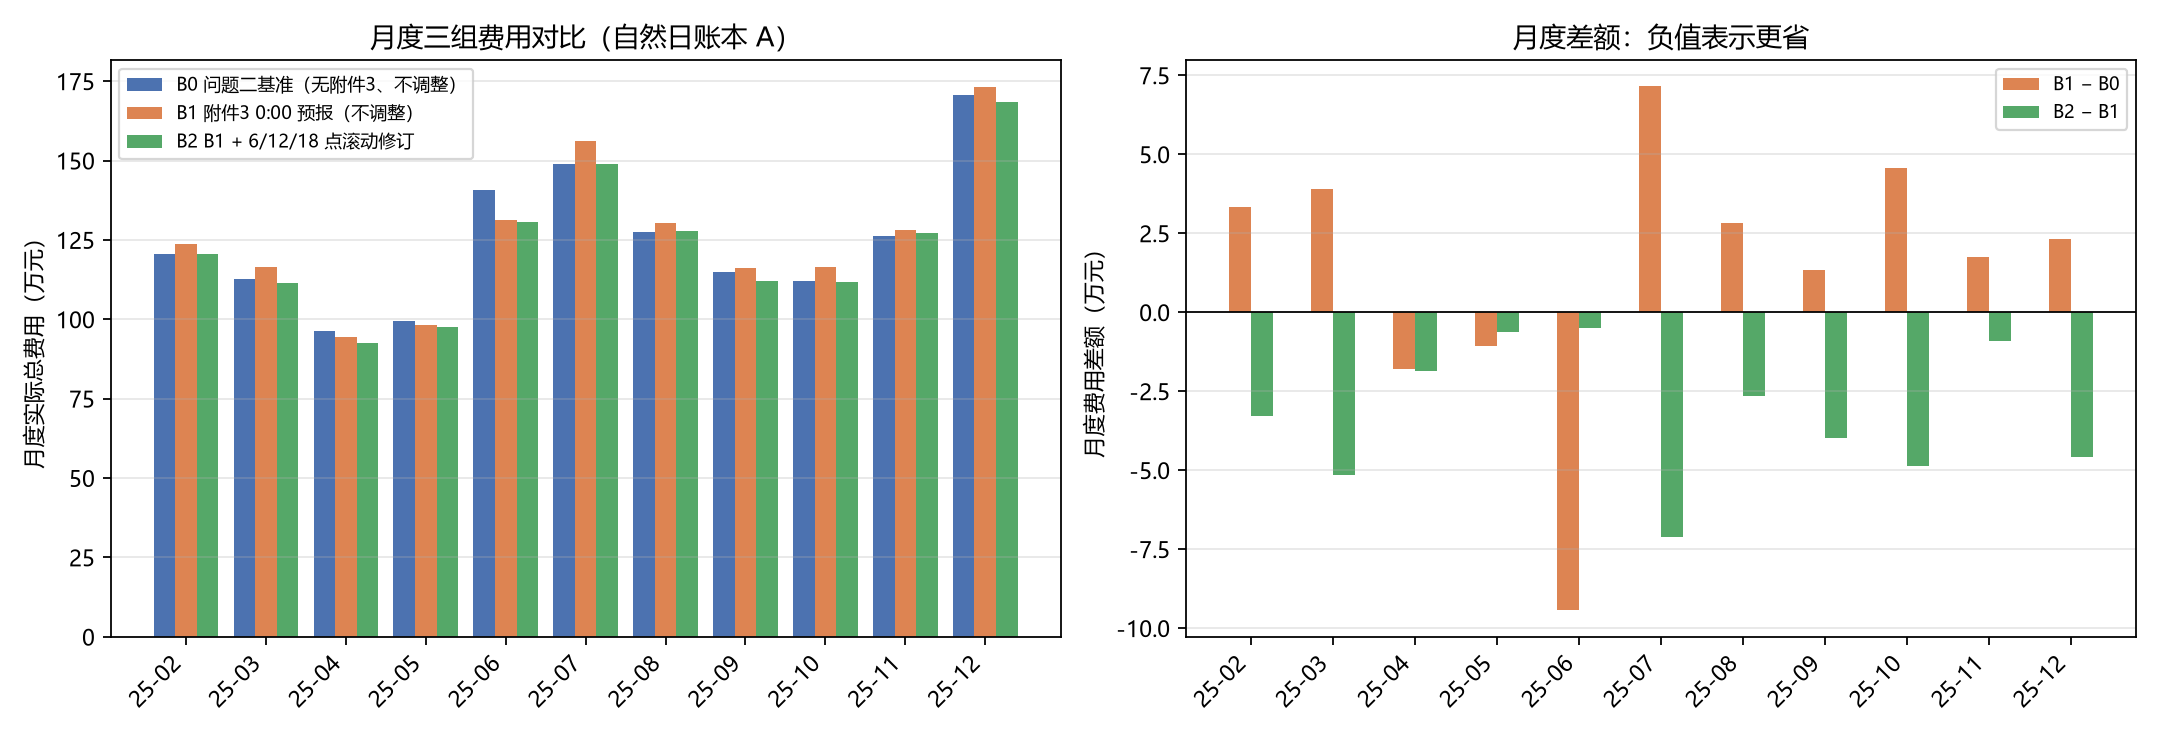
\includegraphics[width=0.88\textwidth]{../../C题/figures/q3_rolling_baseline/monthly_costs.png}
  \caption{三组方案$2025$年$2$--$12$月月度总费用对比}
  \label{fig:q3_monthly_costs}
\end{figure}

$B_2$共执行$1002$次日内更新决策，接受$873$次，各更新节点的决策情况如表~\ref{tab:q3_update_decisions}所示。

\begin{table}[H]
\centering
\caption{$B_2$方案各更新节点的决策与修订电量}
\label{tab:q3_update_decisions}
\zihao{5}
\begin{tabular}{ccccc}
\toprule
\textbf{更新节点} & \textbf{决策数} & \textbf{接受数} & \textbf{接受率} & \textbf{修订电量合计（kWh）} \\
\midrule
$6{:}00$  & $334$ & $334$ & $100.0\%$ & $1\,132\,992$ \\
$12{:}00$ & $334$ & $334$ & $100.0\%$ & $651\,956$ \\
$18{:}00$ & $334$ & $205$ & $61.4\%$  & $18\,097$ \\
\bottomrule
\end{tabular}
\end{table}

\noindent $6{:}00$与$12{:}00$更新全部被接受，修订电量合计超过$178$万~kWh，说明这两个节点的预报携带了显著的新信息；$18{:}00$仅接受$205$次且修订电量只有$18\,097$~kWh，被拒的$129$次对应预测净需求变化恰为$0$，接受的$205$次最大变化也仅$0.098$~kWh。因此$18{:}00$在本轮数据中几乎没有新信息，其价值在于配合前两个节点维持有效版本，不能据此推断应删除该时刻。

按题目要求，表~\ref{tab:q3_purchase_specified}给出$B_2$方案四个指定日期的指定$10$分钟购电量以及全天最终有效购电量与全天总费用。

\begin{table}[H]
\centering
\caption{问题三$B_2$方案指定日期指定时段的最终有效购电量及全天购电量与总费用}
\label{tab:q3_purchase_specified}
\zihao{5}
\begin{tabular}{c|cccccc|cc}
\toprule
\textbf{日期} & $10{:}00$ & $12{:}00$ & $14{:}00$ & $16{:}00$ & $18{:}00$ & $20{:}00$ & \textbf{全天购电量} & \textbf{全天总费用} \\
 & --$10{:}10$ & --$12{:}10$ & --$14{:}10$ & --$16{:}10$ & --$18{:}10$ & --$20{:}10$ & (kWh) & (元) \\
\midrule
3.20 & $0.00$ & $524.61$ & $0.00$ & $492.45$ & $736.39$ & $0.00$ & $66\,900.86$ & $42\,885.68$ \\
6.21 & $0.00$ & $0.00$ & $0.00$ & $151.86$ & $456.69$ & $0.00$ & $34\,873.02$ & $20\,492.59$ \\
9.23 & $0.00$ & $91.47$ & $0.00$ & $456.27$ & $791.07$ & $0.00$ & $68\,226.22$ & $44\,494.94$ \\
12.21 & $0.00$ & $878.59$ & $0.00$ & $837.80$ & $727.88$ & $0.00$ & $96\,121.06$ & $63\,145.63$ \\
\bottomrule
\end{tabular}
\end{table}

\noindent 指定时段购电量取交付前最后一个合法版本的有效购电量，全天购电量与总费用按自然日账本统计。以$3$月$20$日为例，$12{:}00$--$12{:}10$的原始计划为$618.17$~kWh，最终有效购电量为$524.61$~kWh，表明$12{:}00$更新依据最新光伏预报下调了购电量。

表~\ref{tab:q3_storage_1}和表~\ref{tab:q3_storage_2}给出$B_2$方案四个指定日期储能设备六个$4$小时时段的充放电量以及$0{:}00$与$24{:}00$储电量。

\begin{table}[H]
\centering
\caption{问题三$B_2$方案指定日期储能设备前三个$4$小时时段的充放电量及首尾储电量}
\label{tab:q3_storage_1}
\zihao{5}
\begin{tabular}{c|cc|cc|cc|cc}
\toprule
\textbf{日期} & \multicolumn{2}{c|}{$0{:}00$--$4{:}00$} & \multicolumn{2}{c|}{$4{:}00$--$8{:}00$} & \multicolumn{2}{c|}{$8{:}00$--$12{:}00$} & \multicolumn{2}{c}{$0{:}00$ / $24{:}00$储电量} \\
 & 充 & 放 & 充 & 放 & 充 & 放 & (kWh) & (kWh) \\
\midrule
3.20 & $8\,157.56$ & $68.72$ & $1\,784.65$ & $5\,520.57$ & $3\,639.20$ & $3\,232.24$ & $2\,053.71$ & $1\,729.90$ \\
6.21 & $731.38$ & $53.34$ & $1\,302.83$ & $1\,719.95$ & $9\,199.93$ & $0.00$ & $2\,659.60$ & $3\,045.09$ \\
9.23 & $8\,815.73$ & $17.69$ & $1\,445.05$ & $5\,815.55$ & $5\,104.32$ & $2\,387.94$ & $1\,632.41$ & $1\,636.19$ \\
12.21 & $8\,522.89$ & $166.44$ & $2\,388.00$ & $685.44$ & $4\,470.68$ & $8\,392.01$ & $1\,926.74$ & $1\,798.21$ \\
\bottomrule
\end{tabular}
\end{table}

\begin{table}[H]
\centering
\caption{问题三$B_2$方案指定日期储能设备后三个$4$小时时段的充放电量}
\label{tab:q3_storage_2}
\zihao{5}
\begin{tabular}{c|cc|cc|cc}
\toprule
\textbf{日期} & \multicolumn{2}{c|}{$12{:}00$--$16{:}00$} & \multicolumn{2}{c|}{$16{:}00$--$20{:}00$} & \multicolumn{2}{c}{$20{:}00$--$24{:}00$} \\
 & 充 & 放 & 充 & 放 & 充 & 放 \\
\midrule
3.20 & $7\,141.19$ & $254.72$ & $251.26$ & $4\,923.09$ & $521.05$ & $3\,702.95$ \\
6.21 & $0.00$ & $0.00$ & $175.26$ & $4\,968.63$ & $1\,072.58$ & $3\,021.55$ \\
9.23 & $5\,470.48$ & $404.81$ & $105.91$ & $4\,881.21$ & $522.25$ & $3\,875.03$ \\
12.21 & $8\,631.37$ & $2\,220.65$ & $8.16$ & $4\,865.44$ & $471.38$ & $3\,624.59$ \\
\bottomrule
\end{tabular}
\end{table}

\noindent 从储电量变化看，$6$月$21$日光伏充足，日末储电升至$3\,045.09$~kWh；$12$月$21$日冬季高负载，日末储电降至$1\,798.21$~kWh；$3$月$20$日与$9$月$23$日日末储电分别为$1\,729.90$和$1\,636.19$~kWh。储能始终被用于低谷与光伏富余时段充电、高负载时段放电，与问题一的"谷充峰放"规则一致。图~\ref{fig:q3_selected_dates_soc}给出四个指定日期的储电量变化曲线。

\begin{figure}[H]
  \centering
  
\includegraphics[width=0.88\textwidth]{../../C题/figures/q3_rolling_baseline/selected_dates_soc.png}
  \caption{$B_2$方案四个指定日期的储电量变化曲线}
  \label{fig:q3_selected_dates_soc}
\end{figure}

表~\ref{tab:q3_emergency}给出四个指定日期的紧急购电结果。$6$月$21$日无紧急购电，其余三天紧急购电量分别为$33.32$、$6.37$和$12.92$~kWh，对应紧急购电费分别为$166.21$、$43.00$和$75.03$元。

\begin{table}[H]
\centering
\caption{问题三$B_2$方案指定日期的紧急购电结果}
\label{tab:q3_emergency}
\zihao{5}
\begin{tabular}{cccc}
\toprule
\textbf{日期} & \textbf{紧急购电时段} & \textbf{紧急购电量(kWh)} & \textbf{紧急购电费(元)} \\
\midrule
2025.3.20  & 10:00--10:10 & $33.32$ & $166.21$ \\
2025.6.21  & 无 & $0.00$ & $0.00$ \\
2025.9.23  & 20:30--20:40 & $6.37$ & $43.00$ \\
2025.12.21 & 08:00--08:10 & $12.92$ & $75.03$ \\
\bottomrule
\end{tabular}
\end{table}

\subsubsection{结果分析与验证}

针对题目"是否需要引入其他时刻的预报"，三组对照给出的回答是需要。$B_2$相对$B_1$在$11/11$个月、$233/334$天降低现金总费用，平均每月节省约$3.2$万元，应急电量下降$61.9\%$；其中$6{:}00$与$12{:}00$是信息价值最高的更新节点，$18{:}00$主要起维持有效版本的作用。新增其他发布时刻的收益不能仅凭这四个节点外推，若实际可获得更频繁的预报，应在相同的因果信息边界与结算口径下另行回测。

为验证滚动求解链路的可靠性，本文完成三类精简验证：在结算算例中，设$q^{0}=100$~kWh、$p=1$元/kWh，最终有效电量依次取$0$、$80$、$100$、$120$~kWh时，总费用分别为$50$、$90$、$100$、$130$元，减购与增购边界均与式~\eqref{eq:q3_cash}一致；在$2025$年$6$月$21$日信息边界检查中，对$0{:}00$决策时$28\,131$个未实现真值格、$6{:}00$决策时$28\,094$个未实现真值格按$\times1.05$缩放，并给尚未发布的预报增加$50$~kW后，重建整条预测与保护链路得到的计划与接受决策逐位一致；跨求解器一致性检查中，该日$0{:}00$计划目标值差为$3.6\times10^{-12}$元、计划最大差为$2.3\times10^{-13}$~kWh。逐段结算恒等式残差不超过$9.1\times10^{-13}$元，实际储能物理守恒残差不超过$4.6\times10^{-12}$~kWh。

需要说明的是：$B_2$相对$B_1$的节费是"新预报、真实库存反馈与重新优化机会"三者的机制包价值，没有单独隔离预报信息价值；$q_{80}$与自由末态沿用问题二确认口径，分别作为匹配基准与终端约定，不宣称其在第三问调整价格下全局最优。以上限制不影响本文针对题目给出的结论：在当前附件3的四个发布时刻下，引入其他时刻的预报并执行滚动购电调整是值得的。

\subsection{问题四模型建立及求解}

\begin{figure}[H]
  \centering
  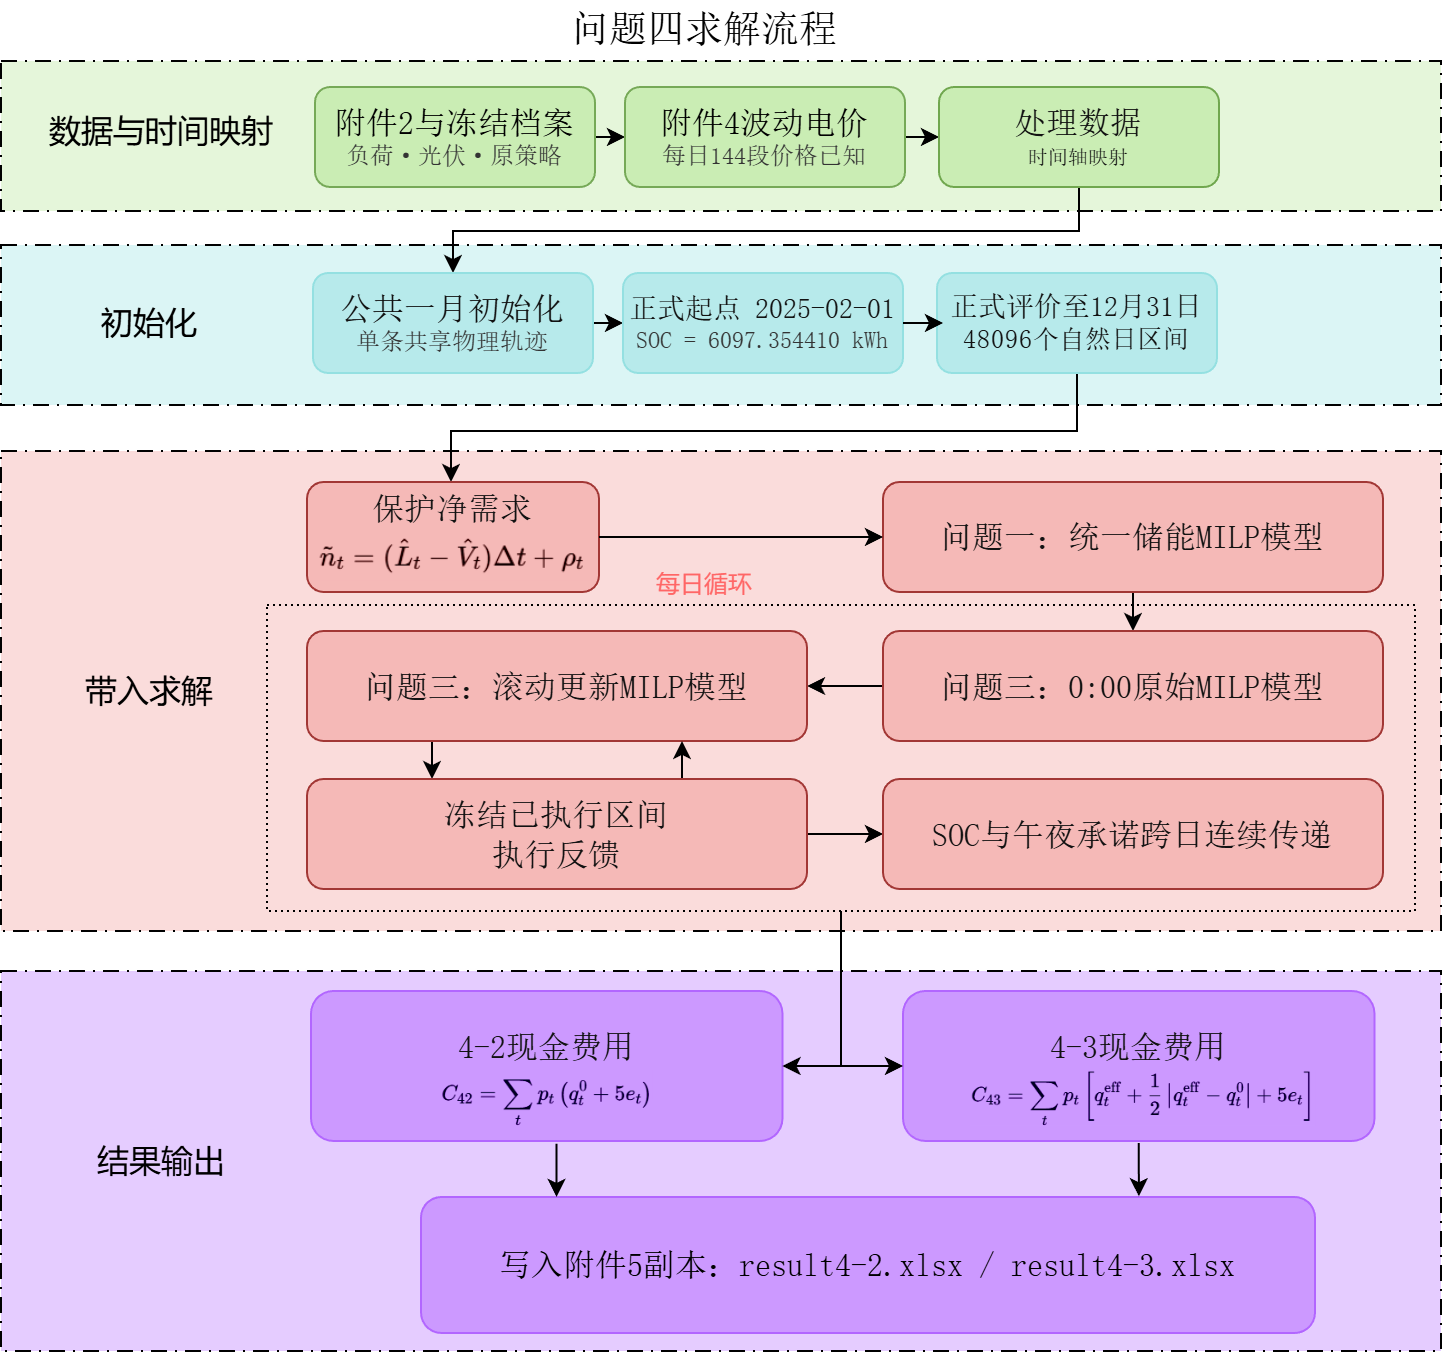
\includegraphics[width=0.9\textwidth]{../../C题/问题四可能用到的图片/问题四求解流程.drawio.png}
  \caption{问题四模型求解流程}
  \label{fig:q4_solution_flow}
\end{figure}


\section{模型的评价与推广}

\subsection{模型的优点}

\begin{enumerate}[label=\arabic*.]
\item 模型以母线功率平衡和储能运行约束为基础，刻画了购电、充放电、弃电与储电状态之间的物理关系，并通过充放电状态变量保证同一时段内储能设备只能充电或放电，使调度方案具有强可执行性。
\item 问题二的模型先基于历史规律预测当日负载与光伏功率，再结合历史预测残差对净需求进行修正；随后据此制定日前购电计划，并在实际运行中依据真实供需逐时段调整储能和应急购电策略，有效降低预测误差的影响，全年调度结果具有较高的可靠性。
\item 问题三在问题二基础上引入光伏预报版本管理和滚动购电修订，通过多版本计划比较与最终一次结算避免中间版本重复计费，并用三组对照定量回答了是否需要引入其他时刻的预报，模型的可扩展性与实际可操作性均得到增强。
\end{enumerate}

\subsection{模型的缺点}

\begin{enumerate}[label=\arabic*.]
  \item 模型将储能设备的充放电效率视为常数，未考虑效率随充放电功率和储电状态变化的非线性特性，可能使计算结果与实际运行存在一定偏差。
  \item 模型未考虑储能设备的循环老化、自放电及运行维护成本，在长期运行场景下，优化结果可能低估实际总费用。
\end{enumerate}

\subsection{模型的推广}

当场景中增加储能设备数量、分布式能源种类或可参与调度的柔性负荷时，只需补充相应的决策变量和约束，即可将模型扩展为规模更大的微网综合能源调度模型。将该框架与预测更新和滚动优化相结合，还可进一步用于光伏、风电等出力不确定条件下的长期调度决策。


% ======================== 参考文献 ========================
\newpage
\begin{thebibliography}{99}
\addcontentsline{toc}{section}{参考文献}

\bibitem{huangfu2018parallelizing} Huangfu Q, Hall J A J. Parallelizing the dual revised simplex method[J]. Mathematical Programming Computation, 2018, 10(1): 119-142.

\end{thebibliography}


% ======================== 附录 ========================
\newpage
\appendix
\renewcommand{\thesection}{附录 \Alph{section}}
\renewcommand{\thesubsection}{\Alph{section}.\arabic{subsection}}
\renewcommand{\thesubsubsection}{\Alph{section}.\arabic{subsection}.\arabic{subsubsection}}
\titleformat{\section}
  {\centering\heiti\zihao{-3}\bfseries}
  {\thesection}{1em}{}

\section{支撑文件列表}

\begin{table}[H]
\centering
\zihao{5}
\begin{tabular}{lll}
\toprule
文件名 & 类型 & 说明 \\
\midrule
03\_q1\_milp.py & Python & 问题一MILP模型求解代码 \\
result1\_baseline.xlsx & Excel & 问题一最优购电策略结果文件 \\
\bottomrule
\end{tabular}
\end{table}


\end{document}
